%%%%%%%%%%%%%%%%%%%%%%%%%
% Dokumentinformationen %
%%%%%%%%%%%%%%%%%%%%%%%%%
\newcommand{\titleinfo}{Elekrizit\"atslehre 4 - Formelsammlung}
\newcommand{\authorinfo}{F. Braun, L. Schmid, U. Giger, R. Koller, S.
Arnold, S. Ferreti}
\newcommand{\versioninfo}{$Revision: 954 $ - powered by \LaTeX}

%%%%%%%%%%%%%%%%%%%%%%%%%%%%%%%%%%%%%%%%%%%%%
% Standard projektübergreifender Header für
% - Makros 
% - Farben
% - Mathematische Operatoren 
%
% DORT NUR ERGÄNZEN, NICHTS LÖSCHEN
%%%%%%%%%%%%%%%%%%%%%%%%%%%%%%%%%%%%%%%%%%%%%  
% Genereller Header
\documentclass[10pt,twoside,a4paper,fleqn]{article}
\usepackage[utf8]{inputenc}
\usepackage[left=1cm,right=1cm,top=1cm,bottom=1cm,includeheadfoot]{geometry}
\usepackage[ngerman]{babel,varioref}

% Pakete
\usepackage{amssymb,amsmath,fancybox,graphicx,color,lastpage,wrapfig,fancyhdr,hyperref,verbatim,floatflt,pxfonts}
\usepackage{esint} %double integral with a circle around

%%%%%%%%%%%%%%%%%%%%
% Generelle Makros %
%%%%%%%%%%%%%%%%%%%%
\newcommand{\formelbuch}[1]{$_{\textcolor{red}{\mbox{\small{S#1}}}}$}
\newcommand{\verweis}[2]{\small{(siehe auch \ref{#1}, #2 (S. \pageref{#1}))}}
\newcommand{\subsubadd}[1]{\textcolor{black}{\mbox{#1}}}


\newcommand{\skriptsection}[2]{\section{#1 {\tiny Skript S. #2}}}
\newcommand{\skriptsubsection}[2]{\subsection{#1 {\tiny Skript S. #2}}}
\newcommand{\skriptsubsubsection}[2]{\subsubsection{#1 {\tiny Skript S. #2}}}

\newcommand{\jom}{j \omega}
%Zeichnet einen 3D-Vektor als Matrix
\newcommand{\ddvector}[3]{\left(\begin{array}{c}#1\\#2\\#3\end{array}\right)} 
%%%%%%%%%%
% Farben %
%%%%%%%%%%
\definecolor{black}{rgb}{0,0,0}
\definecolor{red}{rgb}{1,0,0}
\definecolor{white}{rgb}{1,1,1}
\definecolor{grey}{rgb}{0.8,0.8,0.8}
\definecolor{darkgrey}{rgb}{0.4,0.4,0.4}
\definecolor{orange}{rgb}{0.98,0.5,0.03}

%%%%%%%%%%%%%%%%%%%%%%%%%%%%
% Mathematische Operatoren %
%%%%%%%%%%%%%%%%%%%%%%%%%%%%
\DeclareMathOperator{\sinc}{sinc}



% Fouriertransformationen
\unitlength1cm
\newcommand{\FT}
{
\begin{picture}(1,0.5)
\put(0.2,0.1){\circle{0.14}}\put(0.27,0.1){\line(1,0){0.5}}\put(0.77,0.1){\circle*{0.14}}
\end{picture}
}


\newcommand{\IFT}
{
\begin{picture}(1,0.5)
\put(0.2,0.1){\circle*{0.14}}\put(0.27,0.1){\line(1,0){0.45}}\put(0.77,0.1){\circle{0.14}}
\end{picture}
}

\usepackage{pgfplots}


% Zeilenhöhe Tabellen:
\newcommand{\arraystretchOriginal}{1.5}
\renewcommand{\arraystretch}{\arraystretchOriginal}

\usepackage{tikz}
\usetikzlibrary{circuits.ee.IEC}

%%%%%%%%%%%%%%%%%%%%%%%%%%%%
% Allgemeine Einstellungen %
%%%%%%%%%%%%%%%%%%%%%%%%%%%%
%pdf info
\hypersetup{pdfauthor={\authorinfo},pdftitle={\titleinfo},colorlinks=false}
\author{\authorinfo}
\title{\titleinfo}

%Kopf- und Fusszeile
\pagestyle{fancy}
\fancyhf{}
%Linien oben und unten
\renewcommand{\headrulewidth}{0.5pt} 
\renewcommand{\footrulewidth}{0.5pt}

\fancyhead[L]{\titleinfo{ }\tiny{(\versioninfo)}}
%Kopfzeile rechts bzw. aussen
\fancyhead[R]{Seite \thepage { }von \pageref{LastPage}}
%Fusszeile links bzw. innen
\fancyfoot[L]{\footnotesize{\authorinfo}}
%Fusszeile rechts bzw. ausen
\fancyfoot[R]{\footnotesize{\today}}

% Einrücken verhindern versuchen
\setlength{\parindent}{0pt}



%%%%%%%%%%%%%%%%%%%%%%%%%%%%%%%%%%%%%%%%%%%%%
%% Aus altem Header
\usepackage{esint} %double integral with a circle around
\usepackage{tikz}
\usepackage{pgfplots}
\usepgflibrary{shapes.misc}
\usepackage{circuitikz}

\newcommand{\jom}{j \omega} % Deprecated!
%Zeichnet einen 3D-Vektor als Matrix
\newcommand{\ddvector}[3]{\left(\begin{array}{c}#1\\#2\\#3\end{array}\right)} % Deprecated!



%%%%%%%%%%%%%%%%%%%%%%%%%%%%%%%%%%%%%%%%%%%%
% Möglichst keine Ergänzungen hier, sondern in header.tex
\begin{document} 
 

%%%%%%%%%%%%%%%%%%%%%%%%%%%%%%%%%%%%%%%%%%%%%%%%%%%%%%%%%%%%%%%%%%%%%%%%%%%%%%%%%%%%%%%%%%%%%%%
%%%%%%%%%%%%%%%%%%%%%%%%%%%%%%%%%%%%%%%%%%%%%%%%%%%%%%%%%%%%%%%%%%%%%%%%%%%%%%%%%%%%%%%%%%%%%%%

\section{Schwingkreise}
\subsection{Freie Schwingung}
Die Werte $\textcolor{blue}{U_1,U_2,\beta_u}\text{ sowie
}\textcolor{red}{I_1,I_2,\beta_i}$ müssen aus den Anfangswerten bestimmt
werden.\\
\renewcommand{\arraystretch}{2.5}
\begin{tabular}{| p{4cm} | p{7cm} | p{7cm} |}
	\hline
		& \textbf{Parallelschwingkreis} 
		& \textbf{Serienschwingkreis} \\
	\hline
	& \begin{tikzpicture}[circuit ee IEC, x=2cm, y=2cm, semithick]
	\node (topR) [contact] at (0,1) {};
	\node (bottomR) [contact] at (0,0) {};
	\node at (0,1.2) {};
	
	\draw (topR) to [current direction={very near start, info=$i_R$},
					 resistor={info=R}] (bottomR);
	\draw (topR) -- ++(left:1) 
		to [current direction={very near start, info=$i_L$},
		    inductor={info=L}] ++(down:1)
		-- +(right:1);
	\draw (topR) -- ++(right:1)
		to [current direction={very near start, info=$i_C$},
		    capacitor={info=C}] ++(down:1)
		-- +(left:1);
	\draw[-to, shorten <= 0.2cm,shorten >=0.2cm] (-1.2,1) 
		to node[anchor=east] {$u(t)$} (-1.2,0);
\end{tikzpicture}
	& \begin{circuitikz}[scale=2, european, american inductors]
\ctikzset{bipoles/length=1.2cm}
	\draw
	(0,0)
		to[L=L, o-](1,0)
	(1,0) to[R=R](2,0)
	(2,0) to[C=C, -o](3,0);
\end{circuitikz}


% \begin{tikzpicture}[circuit ee IEC, x=2cm, y=2cm, semithick]
% 	\node (start) [contact] at (0,0) {};
% 	\node (end) [contact] at (3,0) {};
% 	\draw (start) to [inductor={info=L}] (1,0)
% 				  to [resistor={info=R}] (2,0) 
% 				  to [capacitor={info=C}](3,0)
% 				  -- (end);
% 	
% 	\node (placeholder1) at (0,0.5) {};
% 	\node (placeholder2) at (0,-0.5) {};	
% \end{tikzpicture}

% Die Nodes placeholder1 und placeholder2 sind nur dazu da, damit die ganze
% Abbildung wieder gleich hoch ist wie der Parallel-Schwingkreis (siehe
% ParallelSK.tex)
\\
	\hline
%		& \parbox{7cm}{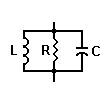
\includegraphics[height=2cm]{../El4/bilder/lcrpara.jpg}}
%		& \parbox{7cm}{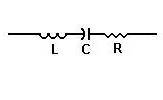
\includegraphics[height=2cm]{../El4/bilder/lcrseries.jpg}} \\
%	\hline	
	DGL &
  $\ddot{u} + \dfrac{1}{RC} \dot{u} + \dfrac{1}{LC} u = 0$
  & $\ddot{i} + \dfrac{R}{L} \dot{i} + \dfrac{1}{LC} i = 0$\\
  & $\ddot{u} + \dfrac{\omega_r}{Q_P} \dot{u} + \omega_r^2 u = 0$
  & $\ddot{i} + \dfrac{\omega_r}{Q_S} \dot{i} + \omega_r^2 i = 0$\\
	\hline
	Resonanzfrequenz & \multicolumn{2}{|c|}{$\omega_r =
	\frac{1}{\sqrt{LC}}$} \\
	\hline
	Güte & 
	$Q_P = R\sqrt{\frac{C}{L}} = \frac{R}{\omega_r L}=R\omega_rC$ &
	$Q_S = \frac{1}{R}\sqrt{\frac{L}{C}} = \frac{\omega_r
	L}{R}=\frac{1}{R\omega_rC}$\\
	\hline
	Dämpfungsfaktor & \multicolumn{2}{|c|}{$\xi=\frac{1}{2Q}$} \\
	\hline
	
	\textcolor{darkgrey}{Standardstartbedingungen} &
	\begin{minipage}{7cm}
    	\vspace{0.1cm}
    	\textcolor{darkgrey}{$u(t=0)=U_0$\quad
    	$\dot{u}(t=0)=-\dfrac{U_o}{RC}$}\\
    \end{minipage} &
	\begin{minipage}{7cm}
     	\vspace{0.1cm}
    	\textcolor{darkgrey}{$i(t=0)=0$\quad
    	$\dot{i}(t=0)=\dfrac{U_o}{L}$}\\   
    \end{minipage}\\
	\hline
	Aperiodisch, $ Q < \frac{1}{2}$
		& $u(t) = \textcolor{blue}{U_1} e^{\alpha_1 t} + \textcolor{blue}{U_2} e^{\alpha_2 t}$ 
		& $i(t) = \textcolor{red}{I_1} e^{\alpha_1 t} + \textcolor{red}{I_2} e^{\alpha_2 t}$ \\
		& $\alpha_{1,2} = - \frac{\omega_r}{2 Q_P} \pm \omega_r \sqrt{\frac{1}{4 Q_P^2} - 1}$	
		& $\alpha_{1,2} = - \frac{\omega_r}{2 Q_S} \pm \omega_r \sqrt{\frac{1}{4Q_S^2} - 1}$\\
		& \textcolor{darkgrey}{$U_1 = U_0 \frac{\frac{\omega_r}{Q} +
		\alpha_2}{\alpha_2 - \alpha_1} \quad$ $U_2 = U_0 \frac{\frac{\omega_r}{Q} +
		\alpha_1}{\alpha_1 - \alpha_2}$}
		& \textcolor{darkgrey}{$I_1 = \frac{U_0}{(\alpha_1 - \alpha_2)L} \quad I_2
		= -I_1$}
		\vspace{0.1cm}
		\\
	\hline 	
	Kritisch, $ Q = \frac{1}{2}$
		& $u(t) = (\textcolor{blue}{U_1} + \textcolor{blue}{\beta_u} t) 
		e^{\alpha t} = (\textcolor{blue}{U_1} + \textcolor{blue}{\beta_u} t) 
		e^{- \omega_r t}$ 
		& $u(t) = (\textcolor{red}{I_1} + \textcolor{red}{\beta_i} t) 
		e^{\alpha t} = (\textcolor{red}{I_1} + \textcolor{red}{\beta_i} t) 
		e^{- \omega_r t}$ \\
% 		& $i(t) = \textcolor{red}{I_1} e^{- \omega_r t} +
% 		\textcolor{red}{\beta_i} t e^{- \omega_r t}$ \\ 
		& $\alpha_{1,2} = - \dfrac{\omega_r}{2 Q_P} = - \omega_r$ & 
		$\alpha_{1,2} = - \dfrac{\omega_r}{2 Q_S} = - \omega_r$\\
		& \textcolor{darkgrey}{$U_1 = U_0 \quad \beta = -U_0 \left(
		\frac{\omega_r}{Q}+\alpha \right)$} & 
		\textcolor{darkgrey}{$I_1 = 0 \quad \beta = \dfrac{U_0}{L}$}
		\vspace{0.1cm}
		\\
	\hline 	
	Periodisch, $ Q > \frac{1}{2}$
		& $u(t) = \textcolor{blue}{U_1} e^{\alpha_1 t} + 
					\textcolor{blue}{U_2} e^{\alpha_2 t} $
		& $i(t) = \textcolor{red}{I_1} e^{\alpha_1 t} + 
					\textcolor{red}{I_2} e^{\alpha_2 t} $ \\
% 	 	& $i(t) = \textcolor{red}{I_1} e^{-\frac{\omega_r}{2 Q_S} t} \cos{\omega_0 t} + 
% 					\textcolor{red}{I_2} e^{-\frac{\omega_r}{2 Q_S} t} \sin{\omega_0 t} $ \\
		& $\alpha_{1,2} = - \frac{\omega_r}{2 Q_P} \pm j \omega_r \sqrt{1 - \frac{1}{4 Q_P^2}}$	
		& $\alpha_{1,2} = - \frac{\omega_r}{2 Q_S} \pm j \omega_r \sqrt{1 - \frac{1}{4 Q_S^2}}$	\\
		& $\omega_0 = \omega_r \sqrt{1 - \frac{1}{4 Q_P^2}} \qquad \omega_0 \approx \omega_r (Q_P > 10)$ 
		& $\omega_0 = \omega_r \sqrt{1 - \frac{1}{4 Q_S^2}} \qquad \omega_0 \approx\omega_r (Q_S > 10)$\\
		& \textcolor{darkgrey}{$u(t) = \frac{U_0 \omega_r}{\omega_0} e^{- \frac{\omega_r}{2
					Q} t} \cos{[\omega_0 t + \arctan{\frac{1}{\sqrt{4 Q^2 -1}}}]}$}
		& \textcolor{darkgrey}{$I_1 =  \frac{U_0}{L \cdot 2 \cdot j \omega_0} \quad I_2 = -I_1$
		$ \quad i(t) = \frac{U_0}{\omega_0 L} e^{-\xi  \omega_r  t} \sin{(\omega_0 t)}$}
		%%\vspace{0.1cm}
		\\
	\hline
	\end{tabular}
	
\renewcommand{\arraystretch}{\arraystretchOriginal}


\subsection{Erzwungene Schwingung}	


\begin{tabular}{|p{4cm}|p{2.4cm}|p{2.4cm}|p{2.4cm}|p{2.4cm}|p{2.4cm}|p{2.4cm}|}
	\hline
		Maximalwerte &
		\multicolumn{3}{|l|}{$I_{Lmax}=I_{Cmax}=\dfrac{I\cdot
   		Q_P}{\sqrt{1-\frac{1}{4Q_P}}}$} &
   	\multicolumn{3}{|l|}{Gilt auch für $U_{Lmax}=U_{Cmax}$ bei
   		dem Serieschwing- } \\
    & \multicolumn{3}{|l|}{$\omega_{I_{Lmax}} =
   		\omega_r\sqrt{1-\frac{1}{2Q_P^2}}\qquad \omega_{I_{Cmax}} =
   		\dfrac{\omega_r}{\sqrt{1-\frac{1}{2Q_P^2}}}$} &
   		\multicolumn{3}{|l|}{kreis, jedoch muss $Q_P$ mit $Q_s$ ersetzt werden.}\\
   \hline
   	Bandbreite, Verstimmung 
   	&
		\multicolumn{3}{|l|}{
			\begin{minipage}[c]{6cm}
			\pgfmathdeclarefunction{gauss}{2}{%
  \pgfmathparse{1/(#2*sqrt(2*pi))*exp(-((x-#1)^2)/(2*#2^2))}%
}

\makebox{\begin{tikzpicture}[scale=0.6, every node/.style={scale=0.6}]
\begin{axis}[
  no markers,
  domain=0:6,
  samples=500,
  hide x axis=true,
	hide y axis=true,
  %height=5cm, width=12cm,
  %xtick={4,6.5}, ytick=\empty,
  enlargelimits=false,
  clip=false,
  axis on top,
  grid = major
  ]
  \addplot {gauss(3,1)};
\end{axis}

	\draw[->, thick] (-0.2,0) -- +(right:7.5) node[right] {$\omega$};
	\draw (2.43,1pt) -- (2.43,-1pt) node[anchor=north] {$\omega_1$};%
	\draw (3.43,1pt) -- (3.43,-1pt) node[anchor=north] {$\omega_r$};%
	\draw (4.43,1pt) -- (4.43,-1pt) node[anchor=north] {$\omega_2$};%

	\draw[->, thick] (0,-0.2) -- +(north:6.5) node[above] {$P$};
	\draw (0.05,3.85) -- (-0.05,3.85) node[anchor=east] {$\frac{Max}{2}$};
	\draw (0.05,5.7) -- (-0.05,5.7) node[anchor=east] {$Max$};

	\draw[->] (1,-0.2) -- +(north:6.5) node[above] {$U/I/Z(\omega)$};
	\draw (1.05,3.85) -- (0.95,3.85) node[anchor=east] {$\frac{Max}{\sqrt{2}}$};
	\draw (1.05,5.7) -- (0.95,5.7) node[anchor=east] {$Max$};

	\draw[dashed] (1,3.85) -- (4.5,3.85);
	\draw[dashed] (1,5.7) -- (3.55,5.7);
	\draw[dashed, shorten <= -3pt] (2.43,4) -- (2.43,0);
	\draw[dashed, shorten <= -3pt] (3.43,5.75) -- (3.43,0);
	\draw[dashed, shorten <= -3pt] (4.43,4) -- (4.43,0);


\end{tikzpicture}}




% \pgfmathdeclarefunction{gauss}{2}{
%   \pgfmathparse{7.5/(#2*sqrt(2*pi))*exp(-((x-#1)^2)/(2*#2^2))}
% }
% 
% \begin{tikzpicture}
% \begin{axis}[every axis plot post/.append style={
% 	 	  mark=none,
% 	 	  domain=0:6,
% 	 	  samples=40,
% 	 	  smooth,
% 	 	  no marks},
% 	 	  hide x axis=true,
% 	 	  hide y axis=true,
% 	 	  enlargelimits=upper]
% 	  \addplot {gauss(0,0.5)};
% 	  \addplot {gauss(3,0.75)};
% 	\end{axis}
% 	\draw[->, very thick] (-0.2,0) -- +(right:6) node[right] {$\omega$};
% 	\draw (2,1pt) -- (2,-1pt) node[anchor=north] {$\omega_1$};
% 	\draw (3,1pt) -- (3,-1pt) node[anchor=north] {$\omega_r$};
% 	\draw (4,1pt) -- (4,-1pt) node[anchor=north] {$\omega_2$};
% 
% 	\draw[->, very thick] (0,-0.2) -- +(north:3.5) node[above] {$P$};
% 	\draw (0.05,2) -- (-0.05,2) node[anchor=east] {$\frac{Max}{2}$};
% 	\draw (0.05,3) -- (-0.05,3) node[anchor=east] {$Max$};
% 
% 	\draw[->] (1,-0.2) -- +(north:3.5) node[above] {$U/I/Z(\omega)$};
% 	\draw (1.05,2) -- (0.95,2) node[anchor=east] {$\frac{Max}{\sqrt{2}}$};
% 	\draw (1.05,3) -- (0.95,3) node[anchor=east] {$Max$};
% 
% 	\draw[dashed] (1,2) -- (4.05,2);
% 	\draw[dashed] (1,3) -- (3.05,3);
% 	\draw[dashed, shorten <= -3pt] (2,2) -- (2,0);
% 	\draw[dashed, shorten <= -3pt] (3,3) -- (3,0);
% 	\draw[dashed, shorten <= -3pt] (4,2) -- (4,0);
% 
% \end{tikzpicture}




% \pgfmathdeclarefunction{gauss}{2}{
%   \pgfmathparse{1/(#2*sqrt(2*pi))*exp(-((x-#1)^2)/(2*#2^2))}
% }

% \begin{tikzpicture}
% 	\begin{axis}[every axis plot post/.append style={
% 	  mark=none,
% 	  domain=0:6,
% 	  samples=10,
% 	  smooth, % All plots: from -2:2, 50 samples,
% 	  no marks},
% 	  hide x axis=true, % no box around the plot, only x and y axis
% 	  hide y axis=true, % the * suppresses the arrow tips
% 	  enlargelimits=upper] % extend the axes a bit to the right and top
% 	\addplot {gauss(3,0.75)}
%   
%   \end{axis}
%   
% 	\draw[->, very thick] (-0.2,0) -- +(right:6) node[right] {$\omega$};
% 	\draw (2,1pt) -- (2,-1pt) node[anchor=north] {$\omega_1$};
% 	\draw (3,1pt) -- (3,-1pt) node[anchor=north] {$\omega_r$};
% 	\draw (4,1pt) -- (4,-1pt) node[anchor=north] {$\omega_2$};
% 
% 	\draw[->, very thick] (0,-0.2) -- +(north:3.5) node[above] {$P$};
% 	\draw (0.05,2) -- (-0.05,2) node[anchor=east] {$\frac{Max}{2}$};
% 	\draw (0.05,3) -- (-0.05,3) node[anchor=east] {$Max$};
% 
% 	\draw[->] (1,-0.2) -- +(north:3.5) node[above] {$U/I/Z(\omega)$};
% 	\draw (1.05,2) -- (0.95,2) node[anchor=east] {$\frac{Max}{\sqrt{2}}$};
% 	\draw (1.05,3) -- (0.95,3) node[anchor=east] {$Max$};
% 
% 	\draw[dashed] (1,2) -- (4.05,2);
% 	\draw[dashed] (1,3) -- (3.05,3);
% 	\draw[dashed, shorten <= -3pt] (2,2) -- (2,0);
% 	\draw[dashed, shorten <= -3pt] (3,3) -- (3,0);
% 	\draw[dashed, shorten <= -3pt] (4,2) -- (4,0);
%   
%   
% \end{tikzpicture}



% \begin{tikzpicture}
% \begin{axis}[every axis plot post/.append style={
% 	mark=none,domain=0:6,samples=50,smooth},
% 	hide x axis=true,
%   hide y axis=true
%   ]

%	\draw[->, very thick] (-0.2,0) -- +(right:6) node[right] {$\omega$};
%	\draw (2,1pt) -- (2,-1pt) node[anchor=north] {$\omega_1$};
% 	\draw (3,1pt) -- (3,-1pt) node[anchor=north] {$\omega_r$};
% 	\draw (4,1pt) -- (4,-1pt) node[anchor=north] {$\omega_2$};
% 	
% 	\draw[->, very thick] (0,-0.2) -- +(north:3.5) node[above] {$P$};
% 	\draw (0.05,2) -- (-0.05,2) node[anchor=east] {$\frac{Max}{2}$};
% 	\draw (0.05,3) -- (-0.05,3) node[anchor=east] {$Max$};
% 	
% 	\draw[->] (1,-0.2) -- +(north:3.5) node[above] {$U/I/Z(\omega)$};
% 	\draw (1.05,2) -- (0.95,2) node[anchor=east] {$\frac{Max}{\sqrt{2}}$};
% 	\draw (1.05,3) -- (0.95,3) node[anchor=east] {$Max$};
% 	
% 	\draw[dashed] (1,2) -- (4.05,2);
% 	\draw[dashed] (1,3) -- (3.05,3);
% 	\draw[dashed, shorten <= -3pt] (2,2) -- (2,0);
% 	\draw[dashed, shorten <= -3pt] (3,3) -- (3,0);
% 	\draw[dashed, shorten <= -3pt] (4,2) -- (4,0);

  
% 	\addplot {gauss(1,0.75)}
% 
% \end{axis}
% \end{tikzpicture}
			\end{minipage}} &
		\multicolumn{3}{|l|}{
			\begin{minipage}[c]{6cm}
  			$b_w = \omega_2 - \omega_1 = \dfrac{\omega_r}{Q}$\\
  			$B = \dfrac{f_r}{Q}=\dfrac{b_w}{2\pi}$\\\\
				$\eta = \dfrac{\omega}{\omega_r} - \dfrac{\omega_r}{\omega} \qquad
				\dfrac{Z}{R} = \dfrac{U}{U_{max}} = \dfrac{1}{\sqrt{1 + (\eta Q)^2}}$
			\end{minipage}}\\
	\hline
		& \multicolumn{2}{|l|}{$\omega = \omega_1$}
		& \multicolumn{2}{|l|}{$\omega = \omega_r$}
		& \multicolumn{2}{|l|}{$\omega = \omega_2$} \\
	\hline
		Zeigerdiagramme &
		\multicolumn{2}{|l|}{\begin{tikzpicture}[scale=0.6, yscale=0.6, thick]
	%Koordinatensystem
	\draw[->] (-0.2,0) -- +(right:6) node[right] {$Re$};
	\draw[->] (0,-3) -- +(north:6) node[above] {$Im$};
	
	%Pfeile
	\draw[->, color=red] (0,0.05) -- +(right:5) node[above right]
	{$\underline{I}$};
	\draw[->] (0,0) -- +(right:2.95) node[above left] {$\underline{U}_R
	= \frac{\underline{U}_0}{\sqrt{2}}$};
	\draw[->] (2.95,0) -- (2.95,3) node[left]
	{$\underline{U}_L$};
	\draw[->]	(3.05,3) -- (3.05,-3) node[right] {$\underline{U}_C$};
	\draw[->] (0,0) -- (3,-3) node[left] {$\underline{U}_0$};
	
	%Winkel
	\draw[->, color = green] (2,0) arc (0:-45:2) node[above = 2]
	{$-45^{\circ}$};

\end{tikzpicture}


} &
		\multicolumn{2}{|l|}{\begin{tikzpicture}
	%Koordinatensystem
	\draw[->, very thick] (-0.2,0) -- +(right:6) node[right] {$Re$};
	\draw[->, very thick] (0,-0.2) -- +(north:3.2) node[above] {$Im$};
	
	%Pfeile
	\draw[->, color=red, very thick] (0,0.05) -- +(right:5) node[above right]
	{$\underline{I}$};
	\draw[->, very thick] (0,0) -- +(right:2.95) node[above left] {$\underline{U}_R
	= \underline{U}_0$};
	\draw[->, very thick] (2.95,0) -- (2.95,3) node[left]
	{$\underline{U}_L$};
	\draw[->, very thick]	(3.05,3) -- (3.05,0) node[above right]
	{$\underline{U}_C$};

\end{tikzpicture}

} &
		\multicolumn{2}{|l|}{\begin{tikzpicture}[scale=0.6, yscale=0.6, thick]
	%Koordinatensystem
	\draw[->] (-0.2,0) -- +(right:6) node[right] {$Re$};
	\draw[->] (0,-0.2) -- +(north:4) node[above] {$Im$};
	
	%Pfeile
	\draw[->, color=red] (0,0.05) -- +(right:5) node[above right]
	{$\underline{I}$};
	\draw[->] (0,0) -- +(right:3) node[below left] {$\underline{U}_R
	= \frac{\underline{U}_0}{\sqrt{2}}$};
	\draw[->] (3,0) -- (3,4) node[left]
	{$\underline{U}_L$};
	\draw[->]	(3.10,4) -- (3.10,3) node[right] {$\underline{U}_C$};
	\draw[->] (0,0) -- (3,3) node[left] {$\underline{U}_0$};
	
	%Winkel
	\draw[->, color = green] (1.5,0) arc (0:45:1.5) node[below = 1]
	{$45^{\circ}$};

\end{tikzpicture}


} \\
	\hline
\end{tabular}

\renewcommand{\arraystretch}{\arraystretchOriginal}

\subsection{Verlustbehafteter Schwingkreis}
Resonanzfrequenz $\omega_r$ tritt dort auf, wo 
$\operatorname{Im} \{ \underline{Y}(\omega) \} =
\operatorname{Im}\{\underline{Z}(\omega) \} = 0$.

\subsection{Resonanzkreis mit realen Elementen}
Umrechnungen Parallel- $\Longleftrightarrow$ Serieschaltungen von L \& R oder C \& R. \\

% Siehe http://www.causa-dura.ch/Scripts/aet\_skript.pdf, seite 121 
\renewcommand{\arraystretch}{1.1}
\begin{tabular}{| p{2cm} | p{8cm} | p{8cm} |}
	\hline
		& \textbf{Parallel $\Rightarrow$ Seriell}  
		& \textbf{Seriell $\Rightarrow$ Parallel} \\
	\hline
		L \& R
		& $ R_S = \dfrac{R_P (\omega L_P)^2}{R_P^2 + (\omega L_P)^2} \qquad 
			L_S = \dfrac{R_P^2 L_P}{R_P^2 + (\omega L_P)^2}  $
		& $ R_P = \dfrac{R_S^2 + (\omega L_S)^2}{R_S} \qquad 
			L_P = \dfrac{R_S^2 + (\omega L_S)^2}{\omega^2 L_S}   $ \\
	\hline	
		C \& R
		& $ R_S = \dfrac{R_P}{1 + (\omega R_P C_P)^2} \qquad 
			C_S = \dfrac{1 + (\omega R_P C_P)^2}{(\omega R_P)^2 C_P}$
		& $ R_P = \dfrac{(\omega C_S R_S)^2 + 1}{(\omega C_S)^2 R_S} \qquad
			C_P = \dfrac{C_S}{1 + (\omega C_S R_S)^2}$\\
	\hline
\end{tabular}
\renewcommand{\arraystretch}{1}



\section{RET - Reaktanz-Eintore}
\subsection{Reaktanzen}
	\begin{tabular}{ll ll}
		\parbox{4cm}{
		\begin{tikzpicture}[scale=0.6, yscale=0.6, thick]
	%Koordinatensystem
	\draw[->] (-0.2,0) -- +(right:4) node[right] {$\omega$};
	\draw[->] (0,-0.2) -- +(north:4) node[above] {$X$};
	\draw (0,0) -- (3,2.5) node[right] {$L$};
\end{tikzpicture}



			%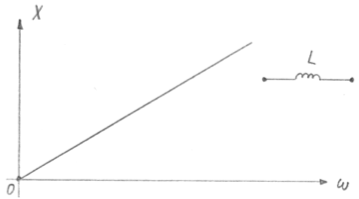
\includegraphics[width=3.5cm]{./images/Induktivitaet}
			}
			& \parbox{5cm}{
				\textbf{Induktivität} \\
				$\underline{Z}=j\omega L \qquad X=\omega L$\\
				$B=-\frac{1}{\omega L}$\\
				Nullstelle: $\lim\limits_{\omega \rightarrow 0} X(\omega) = 0$ \\
				Polstelle: $\lim\limits_{\omega \rightarrow \infty} X(\omega) = \infty$ \\
			}
			
			& \parbox{4cm}{
			\begin{tikzpicture}[scale=0.6, yscale=0.6, thick]
	%Koordinatensystem
	\draw[->] (-0.2,0) -- +(right:4.5) node[right] {$\omega$};
	\draw[->] (0,-3.2) -- +(north:4) node[above] {$X$};
	\draw plot[domain=0.3:4] (\x,{-1/(\x)})
	node[below] {$C$};
\end{tikzpicture}



			%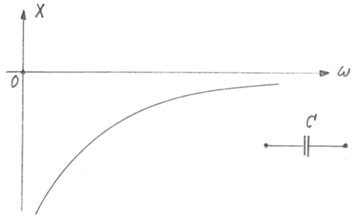
\includegraphics[width=3.5cm]{./images/Kapazitaet}
			}
			& \parbox{5cm}{
				\textbf{Kapazität} \\
				$\underline{Z}=\frac{1}{j\omega C}=\frac{-j}{\omega C} \qquad X=\frac{-1}{\omega C}$\\
				$B=\omega C$ \\
				Nullstelle: $\lim\limits_{\omega \rightarrow \infty} X(\omega) = 0$ \\
				Polstelle: $\lim\limits_{\omega \rightarrow 0} X(\omega) = -\infty$ \\
			}
	\end{tabular}
	
\subsection{Vorgehen bei Netzwerkanalyse}
	\begin{enumerate}{\setlength{\itemsep}{0cm}\setlength{\parsep}{0cm} \setlength{\topsep}{0cm}}
      \item Schaltung übersichtlich aufzeichenen und den Startpunkt der Addition bestimmen
      \item Frequenzverlauf der Reaktanz finden durch fortgeschrittene Addition und Inversion
      \item Inversion: $B(\omega)=\frac{-1}{X(\omega)}$ ; $Polstelle \Longleftrightarrow Nullstelle$
      \item Die so entstandenen Pole und Nullstellen, ausser 0 und $\infty$ sind die Resonanzfrequenzen des RET
    \end{enumerate}
	
	

\renewcommand{\arraystretch}{2}
\begin{sidewaystable}
\subsection{RET-Typen}
\begin{tabular}{|l|l|l|l|l|l|p{1.5cm}|p{1.9cm}|}
\hline
	\textbf{Symbol} &
	\textbf{Typ} &
	\textbf{Reaktanz} &
	\textbf{Impedanzfunktion} &
	\multicolumn{2}{|c|}{\textbf{Eigenschaften}} &
	$\bf \boldsymbol\omega = 0$ \newline $\bf \boldsymbol\omega \rightarrow \boldsymbol\infty$ &
	Zähler (n) \newline	Nenner (m) 
	\\
\hline
	\parbox[c][1.5cm]{1.2cm}{\begin{circuitikz}[scale=2, european, american inductors, yscale=0.4]
\ctikzset{bipoles/length=0.5cm}
\draw (0,0)
	to[L, *-*] (0.7cm,0)
	;	
\end{circuitikz}
} &
	L-Typ &
	\parbox[c][3cm]{5.3cm}{\usepgflibrary{shapes.misc}
\begin{tikzpicture}[smooth, xscale=0.5, yscale=0.5]
% Achsen
\draw[->, thick] (-0.2,0) -- +(8,0) node[right] {$\omega$}; % Horizontal
\draw[->, thick] (0,-2) -- +(0,4) node[above] {$X(\omega)$}; % Vertikal

% Plots
\draw[color=green!70!black, thick] plot[domain=0:1.1] (\x,{tan(\x r)}); % Erster Tan
\draw[color=green!70!black, thick] plot[domain=2.01:4.23] (\x,{tan(\x r)}); % zweiter Tan
\draw[color=green!70!black, thick] plot[domain=4.91:8] (\x,{ (0.25 * \x) -1/(\x -4.6) }); % letzte kurve

% Poolstellen
\draw[dashed, thick, draw=red] (1.57,-2.1) -- +(0,4.2); % Poolstelle 1
\draw[dashed, thick, draw=red] (4.71,-2.1) -- +(0,4.2); % Poolstelle 2
\node[cross out, draw=red, thick] (wr1) at (1.57,0) {};
\node[cross out, draw=red, thick] at (4.71,0) {};


\draw[dashed] plot[domain=0:8] (\x, { 0.25 * \x});
\node (wL) at (6.1,2.4) {$\omega L_\infty$};

% Nullstellen
\node[rounded rectangle, draw=blue, thick] at(0,0) {};
\node[rounded rectangle, draw=blue, thick] at(3.141,0) {};
\node[rounded rectangle, draw=blue, thick] at(5.35,0) {};
\end{tikzpicture}}&
	\begin{tabular}{cl}
	 $ \underline{Z}(p)$ & $ =p\frac{a_np^{n-1}+ \ldots +a_1}{b_mp^m+ \ldots b_0}$
	 \\ 
	 & $=\frac{j\omega
	L_{\infty}[(j\omega)^2+\omega_3^2][\ldots]}{[(j\omega)^2+\omega_2^2][\ldots]}$
	\end{tabular} &
	L-Kreis &
	L-TB &
	Null \newline Pol &
	ungerade \newline $m=n-1$
	\\
\hline
	\parbox[c][1.5cm]{1.2cm}{\begin{circuitikz}[scale=2, european, american inductors, yscale=0.4]
\ctikzset{bipoles/length=0.5cm}
\draw (0,0)
	to[C, *-*] (0.7cm,0)
	;	
\end{circuitikz}
} &
	C-Typ &
	\parbox[c][3cm]{5.3cm}{\usepgflibrary{shapes.misc}
\begin{tikzpicture}[smooth, xscale=0.5, yscale=0.5]
% Achsen
\draw[->, thick] (-0.2,0) -- +(9,0) node[right] {$\omega$}; % Horizontal
\draw[->, thick] (0,-2) -- +(0,4) node[above] {$X(\omega)$}; % Vertikal

% Plots
\draw[color=green!70!black, thick] plot[domain=0.45:2.68] (\x,{tan((\x -1.57) r)}); % Erster Tan
\draw[color=green!70!black, thick] plot[domain=3.58:5.8] (\x,{tan((\x -1.57) r)}); % zweiter Tan
\draw[color=green!70!black, thick] plot[domain=6.78:8.6] (\x,{ ((0.25 * \x) -1/(\x -6.3)) -2 }); % letzte kurve

% Poolstellen
\draw[dashed, thick, draw=red] (3.14,-2.1) -- +(0,4.2); % Poolstelle 1
\draw[dashed, thick, draw=red] (6.28,-2.1) -- +(0,4.2); % Poolstelle 2
\node[cross out, draw=red, thick] (wr1) at (3.14,0) {};
\node[cross out, draw=red, thick] at (6.28,0) {};
\node[cross out, draw=red, thick] at (0,0) {};


\draw[dashed] plot[domain=5:8.7] (\x, { (-1 /(0.04 * \x)) + 2.7 });
\begin{scope}[transform shape, scale=1.7]
	\node (wL) at (2.85,-0.7) {$- \frac{1}{\omega C_\infty}$};
\end{scope}

% Nullstellen
\node[rounded rectangle, draw=blue, thick] at(1.57,0) {};
\node[rounded rectangle, draw=blue, thick] at(4.71,0) {};
\end{tikzpicture}} &
	\begin{tabular}{cl}
	  $\underline{Z}(p)$&
	  $=\frac{1}{p}\frac{a_np^{n}+ \ldots +a_0}{b_mp^{m-1}+\ldots	b_1} $ \\
	  & $=\frac{[(j\omega)^2+\omega_2^2][\ldots]}{j\omega
	  C_{\infty}[(j\omega)^2+\omega_3^2][\ldots]}$	  
	\end{tabular} &
	C-Kreis &	
	C-TB &
	Pol \newline Null &
	gerade \newline $m=n+1$
	\\
\hline
	\parbox[c][1.5cm]{1.2cm}{\begin{circuitikz}[scale=2, european, american inductors, yscale=0.3]
\ctikzset{bipoles/length=0.5cm}
\draw (0,0)
	to[C, *-] (0.35cm,0)
	to[L, -*] (0.7cm,0)
	;	
\end{circuitikz}
} &
	S-Typ &
	\parbox[c][3cm]{5.3cm}{\usepgflibrary{shapes.misc}
\begin{tikzpicture}[smooth, xscale=0.5, yscale=0.5]
% Achsen
\draw[->, thick] (-0.2,0) -- +(9,0) node[right] {$\omega$}; % Horizontal
\draw[->, thick] (0,-2) -- +(0,4) node[above] {$X(\omega)$}; % Vertikal

% Plots
\draw[color=green!70!black, thick] plot[domain=0.45:2.68] (\x,{tan((\x -1.57) r)}); % Erster Tan
\draw[color=green!70!black, thick] plot[domain=3.58:5.8] (\x,{tan((\x -1.57) r)}); % zweiter Tan
\draw[color=green!70!black, thick] plot[domain=7.05:9.5] (\x,{ (0.25 * \x) -1/(\x -6.8) }); % letzte kurve

% Poolstellen
\draw[dashed, thick, draw=red] (3.14,-2.1) -- +(0,4.2); % Poolstelle 1
\draw[dashed, thick, draw=red] (6.28,-2.1) -- +(0,4.2); % Poolstelle 2
\node[cross out, draw=red, thick] (wr1) at (3.14,0) {};
\node[cross out, draw=red, thick] at (6.28,0) {};
\node[cross out, draw=red, thick] at (0,0) {};


\draw[dashed] plot[domain=0.55:3.5] (\x, { (-1 /(0.8* \x))});
\begin{scope}[transform shape, scale=1.7]
	\node (wL) at (1.2,-0.9) {$- \frac{1}{\omega C_0}$};
\end{scope}

\draw[dashed] plot[domain=0:9.6] (\x, { 0.25 * \x});
\node (wL) at (7.5,2.5) {$\omega L_\infty$};

% Nullstellen
\node[rounded rectangle, draw=blue, thick] at(1.57,0) {};
\node[rounded rectangle, draw=blue, thick] at(4.71,0) {};
\node[rounded rectangle, draw=blue, thick] at(7.34,0) {};
\end{tikzpicture}} &
	\begin{tabular}{cl}
	  $\underline{Z}(p)$&
	  $=\frac{1}{p}\frac{a_np^{n}+\ldots+a_0}{b_mp^{m-1}+\ldots
	  b_1}$\\
	  &
	  $=\frac{[L_{\infty}(j\omega)^2+\omega_2^2][(j\omega)^2+\omega_4^2][\ldots]}{j\omega[(j\omega)^2+\omega_3^2]\ldots]}$
	\end{tabular} &
	C-TB &
	L-TB &
	Pol \newline Pol &
	gerade \newline $m=n-1$
	\\
\hline
	\parbox[c][1.5cm]{1.2cm}{\begin{circuitikz}[scale=2, european, american inductors, yscale=0.3]
\ctikzset{bipoles/length=0.5cm}
\draw (0,0)
	to[short, *-] (0.1cm,0)
	(0.1cm,0.5) to[short] (0.1cm,-0.5)
	(0.1cm,0.5) to [L] (0.6cm,0.5)
	(0.1cm,-0.5) to [C] (0.6cm,-0.5)
	(0.6cm,0.5) to [short] (0.6cm,-0.5)
	(0.6cm,0) to [short, -*] (0.7cm,0)
	;	
\end{circuitikz}
} &
	P-Typ &
	\parbox[c][3cm]{5.3cm}{\usepgflibrary{shapes.misc}
\begin{tikzpicture}[smooth, xscale=0.5, yscale=0.5]
% Achsen
\draw[->, thick] (-0.2,0) -- +(9,0) node[right] {$\omega$}; % Horizontal
\draw[->, thick] (0,-2) -- +(0,4) node[above] {$X(\omega)$}; % Vertikal

% Plots
\draw[color=green!70!black, thick] plot[domain=0.01:0.9] (\x, {tan( (\x *1.2) r )        }); % Erster Tan
\draw[color=green!70!black, thick] plot[domain=1.3:3.15] (\x,    {tan( (\x*1.2 -2.7) r)    }); % Erster Tan
\draw[color=green!70!black, thick] plot[domain=3.9:5.75] (\x,  {tan( (\x*1.2 -2.7) r)  }); % zweiter Tan
\draw[color=green!70!black, thick] plot[domain=6.5:8.6] (\x,  { ((0.25 * \x) -1/(\x -6)) -2 }); % letzte kurve

% Poolstellen
\draw[dashed, thick, draw=red] (1,-2.1) -- +(0,4.2); % Poolstelle 1
\node[cross out, draw=red, thick] at (1,0) {};

\draw[dashed, thick, draw=red] (3.4,-2.1) -- +(0,4.2); % Poolstelle 2
\node[cross out, draw=red, thick] at (3.4,0) {};

\draw[dashed, thick, draw=red] (6,-2.1) -- +(0,4.2); % Poolstelle 3
\node[cross out, draw=red, thick] at (6,0) {};

%\node[cross out, draw=red, thick] at (0,0) {};


\draw[dashed] plot[domain=5:8.7] (\x, { (-1 /(0.035 * \x)) + 3.2 });
\node (wC) at (7.5,2) {$- \frac{1}{\omega C_\infty}$};
\draw[->, thick] (7.5,1.2) -- +(-0.5,-1.8);

\draw[dashed] plot[domain=0:2] (\x,{\x});
\node at (2.2,2.4) {$\omega L_0$};


% Nullstellen
\node[rounded rectangle, draw=blue, thick] at(0,0) {};
\node[rounded rectangle, draw=blue, thick] at(2.25,0) {};
\node[rounded rectangle, draw=blue, thick] at(4.86,0) {};
\end{tikzpicture}} &
	\begin{tabular}{cl}
	  $\underline{Z}(p)$&
	  $=p\frac{a_np^{n-1}+\ldots +a_1}{b_mp^m+\ldots b_0}$ \\
	  & $=\frac{j\omega[(j\omega)^2+\omega_3^2][\ldots]}{C_{\infty}[(j\omega)^2+\omega_2^2][(j\omega)^2+\omega_4^2]\ldots]}$
	\end{tabular} &
	C-Kreis & L-Kreis &
	Null \newline Null &
	ungerade \newline $m=n+1$
	\\
\hline
\end{tabular}
\caption[Bestimmung des RET-Typ]{Bestimmung des RET-Typ. Die Bezeichnungen
Klemmentrennbündel und Klemmenkreis wurden abgekürzt zu TB und Kreis. Die
Reaktanzdiagramme sind keinenfalls Masstäblich!}
\label{tab:RETTyp}
\end{sidewaystable}
\renewcommand{\arraystretch}{\arraystretchOriginal}
\newpage		
		
\subsection{Minimalreaktanzeintor (MRET)}
	%RET in MRET wandeln:\\
	\begin{enumerate}{\setlength{\itemsep}{0cm}\setlength{\parsep}{0cm} \setlength{\topsep}{0cm}}
      \item Netzwerk übersichtlich aufzeichnen 
      \item Tor offen; Kreise suchen die nur L oder C enthalten; Ein
      Element des Kreises weglassen, es darf aber kein anderer Zweig stromlos werden. 
      \item Tor kurzgeschlossen; Trennbündel suchen(Knoten an denen nur
      L oder C liegen); Ein Element kurzschliessen, dabei darf kein anderes Element kurzgeschlossen werden.
      \item Die verbleibenden Elemente im MRET haben nicht mehr die
      gleichen Grössen und müssen neu berechnet werden.
    \end{enumerate}
	
	%Anzahl Elemente = Höchste Potenzfunktion $\underline{Z}(p)$
		
			
\subsection{Dualität}
\textbf{Vorgehen}
\begin{enumerate}{\setlength{\itemsep}{0cm}\setlength{\parsep}{0cm} \setlength{\topsep}{0cm}}
	\item Netzwerk ohne Kreuzungen aufzeichnen
	\item In jede Masche (auch in Umfangsmasche) einen dualen Knoten setzen
	\item Knoten von anstossenden Maschen verbinden. Jeder dieser Maschen hat
	gemeinsamen Zweig (dualen Zweig).
	\item In die dualen Zweige die dualen Schaltungselemente einsetzen.
	\item Dualfaktor $D [\Omega]$ wählen und Werte der dualen Netzwerk-Elemente
	bestimmen.
\end{enumerate}

\begin{tabular}{llllllll}
$R'=D^2G$ & $L'=D^2C$ & $\underline{U}'=D\underline{I}$ & $G'=\frac{R}{D^2}$ &
$C'=\frac{L}{D^2}$ & $I'=\frac{\underline{U}}{D}$ & Knoten $\leftrightarrow$
Masche & Stern $\leftrightarrow$ Dreieck \\
$R \leftrightarrow G $ & $C \leftrightarrow L$ & $u \leftrightarrow i$ &
$\underline{Z} \leftrightarrow \underline{Y}$ & & & Parallel $\leftrightarrow$
Serie & Stromquelle $\leftrightarrow$ Spannungsquelle\\
\end{tabular}

\subsection{RET-Synthese}
\begin{multicols}{2}
\subsubsection{Mittels Partialbruchzerlegung}
	\begin{enumerate}
	  \item $F(p)=\frac{2p^6+22p^4+68p^2+48}{3p^5+21p^3+30p}$
	  \item $F(p)$ ausdividieren, falls Zählergrad $>$ Nennergrad
	  \item Nenner des echten Bruches zerlegen und Ansatz bilden
	  $\frac{2}{3}p+\frac{8p^4+48p^2+48}{3p^5+21p^3+30p}=\frac{A}{3p}+\frac{Bp}{p^2+2}+\frac{Cp}{p^2+5}$
		\item Erweitern und Koeffizienten bestimmen $A=\frac{24}{5} \qquad
		B=\frac{8}{9} \qquad C=\frac{8}{45}$
		\item Koeffizienten einsetzen
		$F(p)=\frac{2}{3}p+\frac{1}{\frac{15}{24}p}+\frac{1}{\frac{9}{8}p+\frac{1}{\frac{4}{9}p}}+\frac{1}{\frac{45}{8}p+\frac{1}{\frac{8}{255}p}}$
		\item Schaltung aufzeichnen:	  
	\end{enumerate}
	Impedanzfunktion $Z(p)$\\
	\begin{circuitikz}[scale=2, european, american inductors]
\ctikzset{bipoles/length=1.2cm}
\draw (0,0)
	to [L = $2/3H$, *-] (1,0)
	to [C = $15/24F$, -*] (2,0);
\draw (2,0.5) -- (2,-0.5);
\draw (2,0.5) to [L = $4/9H$] (3,0.5);
\draw (2,-0.5) to [C = $9/8H$] (3,-0.5);
\draw (3,0.5) -- (3,-0.5);
\draw (3,0) to [short, *-*] (3.5,0);
\draw (3.5,0.5) -- (3.5,-0.5);
\draw (3.5,0.5) to [L = $8/225H$] (4.5,0.5);
\draw (3.5,-0.5) to [C = $45/8H$] (4.5,-0.5);
\draw (4.5,0.5) -- (4.5,-0.5);
\draw (4.5,0) to [short, *-*] (5,0);
	;	
\end{circuitikz}\\
	Admittanzfunktion $Y(p)$\\
	\begin{circuitikz}[scale=2, european, american inductors]
\ctikzset{bipoles/length=1.2cm}
\draw (0,0) to [short, *-] (4,0);
\draw (0,-2) to [short, *-] (4,-2);
\draw (1,0) to [C = $2/3F$] (1,-2);
\draw (2,0) to [L = $15/24H$] (2,-2);
\draw (3,0) to [L = $9/8H$] (3,-1) to [C = $4/9F$] (3,-2);
\draw (4,0) to [L = $45/8H$] (4,-1) to [C = $8/225F$] (4,-2);	
\end{circuitikz}\\
\subsubsection{Mittels Kettenbruchzerlegung}
\begin{enumerate}
	\item $F(p)=\frac{2p^6+22p^4+68p^2+48}{3p^5+21p^3+30p}$
	\item $F(p)$ ausdividieren $=\frac{2}{3}p+\frac{8p^4+48p^2+48}{3p^5+21p^3+30p}$
	\item Kehrwert des Restes wieder ausdividieren
	$\frac{2}{3}p+\frac{1}{\frac{3p^5+21p^3+30p}{8p^4+48p^2+48}}=\frac{2}{3}p+\frac{1}{\frac{3}{8}p+\frac{3p^3+12p}{8p^4+48p^2+48}}$
	\item Schritt zwei wiederholen bis kein Rest mehr vorhanden ist
	$F(P)=\frac{2}{3}p+\frac{1}{\frac{3}{8}p+\frac{1}{\frac{8}{3}p+\frac{1}{\frac{3}{16}p+\frac{1}{\frac{16}{3}p+\frac{1}{\frac{1}{16}p}}}}}$
	\item Schaltung aufzeichnen:
\end{enumerate}
Impedanzfunktion $Z(p)$\\
\begin{circuitikz}[scale=1.8, european, american inductors]
\ctikzset{bipoles/length=1.2cm}
\draw (0,0) to [L = $2/3H$, *-] (1,0)
						to [L = $8/3H$] (2,0)
						to [L = $16/3H$] (3,0)
						to [C = $1/16F$] (3,-1)
						to [short, -*] (0,-1);
\draw (1,0) to [C = $3/8F$, *-*] (1,-1);
\draw (2,0)	to [C = $1/16F$, *-*] (2,-1);
\end{circuitikz}\\
Admittanzfunktion $Y(p)$\\
\begin{circuitikz}[scale=1.5, european, american inductors]
\ctikzset{bipoles/length=1.0cm}
\draw (-0.5,0) to [short, *-] (0,0)
			to [L = $3/8H$] (1,0)
			to [L = $3/16H$] (2,0)
			to [L = $1/16H$] (3,0)
			to [short] (3,-1)
			to [short, -*] (-0.5,-1);
\draw (0,0) to [C = $2/3F$, *-*] (0,-1);
\draw (1,0) to [C = $8/3F$, *-*] (1,-1);
\draw (2,0) to [C = $16/3F$, *-*] (2,-1);
\end{circuitikz}\\
\end{multicols}



\newpage

\section{Pol- Nullstellendiagramm}
\subsection{Stabilitätsbedingungen}
\begin{tabular}{ll}
	stabil & alle Polstellen in der linken Halbebene\\
	grenzstabil & alle Polstellen in der linken Halbebene und/oder auf der
	imaginären Achse\\
	instabil & mindestens eine Polstelle in der rechten Halbebene
\end{tabular}\\

\subsection{PN-Diagramm aus $u(t)$}

\begin{tikzpicture}[thick]
	\draw [->] (-3,0) -- (3,0);
	\node at (3,0) [anchor=west] {$\sigma$};
	\draw [->] (0,-3) -- (0,3);
	\node at (0,3) [anchor=south] {$j\omega$};
	\draw [dashed] (0,1) -- (1,1) -- (1,-1) -- (0,-1);
	\draw (-2.5,0) node[shape aspect=1,cross out,draw] {};
	\node at (-2.5,0) [anchor=north] {$-20s^{-1}$};
	\draw (0,2) node[shape aspect=1,cross out,draw] {};
	\node at (0,2) [anchor=west] {$j1000s^{-1}$};
	\draw (1,1) node[shape aspect=1,cross out,draw] {};
	\node at (1,1) [anchor=west] {$j500s^{-1}$};
	\draw (1,-1) node[shape aspect=1,cross out,draw] {};
	\node at (1,-1) [anchor=west] {$-j500s^{-1}$};
	\draw (0,-2) node[shape aspect=1,cross out,draw] {};
	\node at (0,-2) [anchor=west] {$-j1000s^{-1}$};
	\draw [->] (1.5,-0.5) -- (1.1,-0.1);
	\node at (1.5,-0.5) [anchor=west] {$4s^{-1}$};
\end{tikzpicture}\newline
\textbf{Allgemein:} \newline
$u(t)=c_1 e^{q_1 \cdot t}+c_2 e^{q_2\cdot t}+\ldots+c_m e^{q_m \cdot t}\quad
q_i$: Pole\newline 
Bei konjugiert-komplexen Paren: $c_{11}e^{(\sigma_1+j\omega_1
t)}+c_{12}e^{(\sigma_1-j\omega_1 t)}=Ae^{\sigma_1 t}\cos{(\omega_1
t+\varphi)}$\\
\textbf{Beispiel:} \newline
$u(t)=20Ve^{\frac{-t}{50ms}}-15V\cos(1000s^{-1}t+\varphi_{11})+12Ve^{4s^{-1}t}\sin(500s^{-1}t+\varphi_{12})$

Polstellen bei: \\
\begin{align}
	20Ve^{\frac{-t}{50ms}} = 20Ve^{-20s^{-1}t} &\rightarrow \text{Pol bei }
	-20s^{-1}\nonumber\\
	-15V\cos(1000s^{-1}t+\varphi_{11}) &\rightarrow \text{Pol bei }
	0\pm j1000s^{-1}\nonumber\\
	12Ve^{4s^{-1}t}\sin(500s^{-1}t+\varphi_{12}) &\rightarrow \text{Pol bei } (4\pm
	j500)s^{-1}\nonumber
\end{align}


\subsection{Frequenzgang $F(j\omega)$ aus PN-Diagramm}
\begin{tabular}{cp{12cm}}
\parbox[c][5cm]{5.3cm}{\begin{tikzpicture}[thick]
	\draw [->] (-2.5,0) -- (2.5,0);
	\node at (2.5,0) [anchor=west] {$\sigma$};
	\draw [->] (0,-2) -- (0,2);
	\node at (0,2) [anchor=south] {$j\omega$};
	\draw [dashed] (-1,1) -- (1,1) -- (1,-1) -- (-1,-1) -- (-1,1);

	\draw (-2,0) node[shape aspect=1,cross out,draw] {};
	\draw (-1,1) node[shape aspect=1,cross out,draw] {};
	\draw (-1,-1) node[shape aspect=1,cross out,draw] {};
	
	\draw (1,-1) node[shape aspect=1,circle ,draw] {};
	\draw (1,1) node[shape aspect=1,circle ,draw] {};
	\draw (2,0) node[shape aspect=1,circle ,draw] {};

	\node at (-2,0) [anchor=north] {$-\sigma_2$};
	\node at (-1,0) [anchor=north] {$-\sigma_1$};
	\node at (1,0) [anchor=north] {$\sigma_1$};
	\node at (2,0) [anchor=north] {$\sigma_2$};
	
	\node at (0,1) [anchor=north west] {$j\omega$};
	\node at (0,-1) [anchor=north west] {$-j\omega$};
\end{tikzpicture}}
& $z =\text{Nullstelle}\newline
p=\text{Polstelle}\newline
F(j\omega)=K\frac{(s-z_1)(s-z_2)\ldots(s-z_n)}{(s-p_1)(s-p_2)\ldots
(s-p_m)}=K\frac{(j\omega-\sigma_1-j\omega_1)\cdot(j\omega-\sigma_1+j\omega_1)\cdot(j\omega-\sigma_2)}{(j\omega+\sigma_1-j\omega_1)\cdot(j\omega+\sigma_1+j\omega_1)\cdot(j\omega+\sigma_2)}$
\end{tabular}

\subsection{Amplitudengang aus $F\left(j\omega\right)$}
\begin{align}
F(j\omega)&=K\cdot\left|\frac{(j\omega-\sigma_1-j\omega_1)\cdot(j\omega-\sigma_1+j\omega_1)\cdot(j\omega-\sigma_2)}{(j\omega+\sigma_1-j\omega_1)\cdot(j\omega+\sigma_1+j\omega_1)\cdot(j\omega+\sigma_2)}\right| 
&= K \cdot \frac{\left|-\sigma_1+j\left(\omega-\omega_1\right)\right|}{\left|\sigma_1+j\left(\omega-\omega_1\right)\right|} \cdot \frac{\left|-\sigma_1+j\left(\omega+\omega_1\right)\right|}{\left|\sigma_1+j\left(\omega+\omega_1\right)\right|} \cdot \frac{\left|-\sigma_2+j\omega\right|}{\left|\sigma_2+j\omega\right|} \nonumber
\end{align}

\subsection{DGL zu UTF}
Ableitung wird zu $\cdot j \omega$:
\[ \frac{du_2^2}{dt^2} + 3\frac{du_2}{dt} + u_2 = \frac{du_1}{dt} \longrightarrow (j\omega)^2u_2 + 3j\omega u_2 + u_2 = j\omega u_1
\]


\newpage


\section{Vierpole}
\begin{sidewaystable}
\subsection{Vierpolgleichungen und ihre Parameter}
	\begin{minipage}{5cm}
    	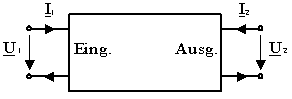
\includegraphics[height=1.5cm]{./bilder/vierpol}
    \end{minipage}
	\begin{minipage}{8cm}
    	Prim. Kurzschluss: $\underline{U}_1=0$ \qquad 
    	Prim. Leerlauf: $\underline{I}_1=0$\\ 
    	Sek. Kurzschluss: $\underline{U}_2=0$ \qquad 
    	Sek. Leerlauf: $\underline{I}_2=0$
    \end{minipage}
		
	\renewcommand{\arraystretch}{1.1}
	\begin{tabular}{| c | c | c | c | c | c | c |}
		\hline
			\textbf{Form}
			& \textbf{Vierpolgleichung} 
			& \textbf{$\Delta_{11}$} 
			& \textbf{$\Delta_{12}$}
			& \textbf{$\Delta_{21}$}
			& \textbf{$\Delta_{22}$}
			& \textbf{Matrixform}\\
		\hline
			\textbf{Impedanzform}
			& $ \begin{matrix}
					\underline{U}_{1}=\underline{Z}_{11}\underline{I}_{1}+\underline{Z}_{12}\underline{I}_{2}\\
					\underline{U}_{2}=\underline{Z}_{21}\underline{I}_{1}+\underline{Z}_{22}\underline{I}_{2}\\
				\end{matrix}$
			& $\underline{Z}_{11}=\frac{\underline{U}_{1}}{\underline{I}_{1}} \mid_{\underline{I}_2=0}$
			& $\underline{Z}_{12}=\frac{\underline{U}_{1}}{\underline{I}_{2}} \mid_{\underline{I}_1=0}$
			& $\underline{Z}_{21}=\frac{\underline{U}_{2}}{\underline{I}_{1}} \mid_{\underline{I}_2=0}$
			& $\underline{Z}_{22}=\frac{\underline{U}_{2}}{\underline{I}_{2}} \mid_{\underline{I}_1=0}$
			& $ \begin{bmatrix}
					\underline{U}_{1}\\
					\underline{U}_{2}\\
				\end{bmatrix}
				=
				\begin{bmatrix}
					Z
				\end{bmatrix}
				\begin{bmatrix}
					\underline{I}_{1}\\
					\underline{I}_{2}\\
				\end{bmatrix}$\\
		\hline
			\textbf{Admittanzform}
			& $ \begin{matrix}
					\underline{I}_{1}=\underline{Y}_{11}\underline{U}_{1}+\underline{Y}_{12}\underline{U}_{2}\\
					\underline{I}_{2}=\underline{Y}_{21}\underline{U}_{1}+\underline{Y}_{22}\underline{U}_{2}\\
				\end{matrix}$
			& $\underline{Y}_{11}=\frac{\underline{I}_{1}}{\underline{U}_{1}} \mid_{\underline{U}_2=0}$
			& $\underline{Y}_{12}=\frac{\underline{I}_{1}}{\underline{U}_{2}} \mid_{\underline{U}_1=0}$
			& $\underline{Y}_{21}=\frac{\underline{I}_{2}}{\underline{U}_{1}} \mid_{\underline{U}_2=0}$
			& $\underline{Y}_{22}=\frac{\underline{I}_{2}}{\underline{U}_{2}} \mid_{\underline{U}_1=0}$
			&$ \begin{bmatrix}
					\underline{I}_{1}\\
					\underline{I}_{2}\\
				\end{bmatrix}
				=
				\begin{bmatrix}
					Y
				\end{bmatrix}
				\begin{bmatrix}
					\underline{U}_{1}\\
					\underline{U}_{2}\\
				\end{bmatrix}$\\
		\hline
			\textbf{Kettenform}
			& $ \begin{matrix}
					\underline{U}_{1}=\underline{A}_{11}\underline{U}_{2}+\underline{A}_{12}\underline{I}_{2}\\
					\underline{I}_{1}=\underline{A}_{21}\underline{U}_{2}+\underline{A}_{22}\underline{I}_{2}\\
				\end{matrix}$
			& $\underline{A}_{11}=\frac{\underline{U}_{1}}{\underline{U}_{2}} \mid_{\underline{I}_2=0}$
			& $\underline{A}_{12}=\frac{\underline{U}_{1}}{\underline{I}_{2}} \mid_{\underline{U}_2=0}$
			& $\underline{A}_{21}=\frac{\underline{I}_{1}}{\underline{U}_{2}} \mid_{\underline{I}_2=0}$
			& $\underline{A}_{22}=\frac{\underline{I}_{1}}{\underline{I}_{2}} \mid_{\underline{U}_2=0}$
			& $ \begin{bmatrix}
					\underline{U}_{1}\\
					\underline{I}_{1}\\
				\end{bmatrix}
				=
				\begin{bmatrix}
					A
				\end{bmatrix}
				\begin{bmatrix}
					\underline{U}_{2}\\
					\underline{I}_{2}\\
				\end{bmatrix}$\\
		\hline
			\textbf{Hybridform}
			& $ \begin{matrix}
					\underline{U}_{1}=\underline{H}_{11}\underline{I}_{1}+\underline{H}_{12}\underline{U}_{2}\\
					\underline{I}_{2}=\underline{H}_{21}\underline{I}_{1}+\underline{H}_{22}\underline{U}_{2}\\
				\end{matrix}$
			& $\underline{H}_{11}=\frac{\underline{U}_{1}}{\underline{I}_{1}} \mid_{\underline{U}_2=0}$
			& $\underline{H}_{12}=\frac{\underline{U}_{1}}{\underline{U}_{2}} \mid_{\underline{I}_1=0}$
			& $\underline{H}_{21}=\frac{\underline{I}_{2}}{\underline{I}_{1}} \mid_{\underline{U}_2=0}$
			& $\underline{H}_{22}=\frac{\underline{I}_{2}}{\underline{U}_{2}} \mid_{\underline{I}_1=0}$
			& $ \begin{bmatrix}
					\underline{U}_{1}\\
					\underline{I}_{2}\\
				\end{bmatrix}
				=
				\begin{bmatrix}
					H
				\end{bmatrix}
				\begin{bmatrix}
					\underline{I}_{1}\\
					\underline{U}_{2}\\
				\end{bmatrix}$\\
		\hline
	\end{tabular}
	\renewcommand{\arraystretch}{\arraystretchOriginal}
	
	\subsection{Spezielle 2-Tore}
	\renewcommand{\arraystretch}{1}
		\begin{tabular}{|l | c | c | c | c|}
			\hline
				&
				& \textbf{Z} 
				& \textbf{Y}
				& \textbf{A}\\
			\hline
				Querimpedanz
				& \ctikzset{bipoles/length=20pt}
\begin{circuitikz}[scale=1, european, american inductors]
	\draw (0,0) to [short, *-*] (2,0);
	\draw (0,-1) to [short, *-*] (2,-1);
	\draw (1,0) to [R=$\underline{Z}_a$] (1,-1);
	\draw (0.3,0.1) rectangle (1.7,-1.1);
	%\node at (1,0.3) [scale=0.7] {Querimpedanz};
\end{circuitikz}
				& $ \begin{bmatrix}
						\underline{Z}_{a} & \underline{Z}_{a} \\
						\underline{Z}_{a} & \underline{Z}_{a} \\
					\end{bmatrix}$
				& -
				& $ \begin{bmatrix}
						1 & 0 \\
						\frac{1}{\underline{Z}_{a}} & 1 \\
					\end{bmatrix}$\\
			\hline
				Längsimpedanz
				& \ctikzset{bipoles/length=20pt}
\begin{circuitikz}[scale=1, european, american inductors]
	\node at (0,0.2) {};
	\node at (0,-0.8) {};
	\draw (0,0) to [short, *-] (0.5,0);
	\draw (1.5,0) to [short, -*] (2,0);
	\draw (0,-0.6) to [short, *-*] (2,-0.6);
	\draw (0.5,0) to [R, l_=$\underline{Z}_a$] (1.5,0);
	\draw (0.3,0.2) rectangle (1.7,-0.7);
	%\node at (1,0.3) [scale=0.7] {Längsimpedanz};
\end{circuitikz}
				& -
				& $ \begin{bmatrix}
						\frac{1}{\underline{Z}_{b}} & -\frac{1}{\underline{Z}_{b}} \\
						-\frac{1}{\underline{Z}_{b}} & \frac{1}{\underline{Z}_{b}} \\
					\end{bmatrix}$
				& $ \begin{bmatrix}
						1 & \underline{Z}_{b} \\
						0 & 1 \\
					\end{bmatrix}$\\
			\hline
				T-Glied
				& \ctikzset{bipoles/length=20pt}
\begin{circuitikz}[scale=1, european, american inductors]
\node at (0,0.2) {};
\node at (0,-1.2) {};
	\draw (0,0) to [short, *-] (0.2,0);
	\draw (0.2,0) to [R, l=$\underline{Z}_1$] (1.2,0);
	\draw (1.2,0) to [R, l=$\underline{Z}_2$] (2.2,0);
	\draw (2.2,0) to [short, -*] (2.5,0);
	\draw (0,-1) to [short, *-*] (2.5,-1);
	\draw (1.2,0) to [R=$\underline{Z}_3$] (1.2,-1);
	%\draw (0.2,0.2) rectangle (2.2,-1.1);
	%\node at (1,0.5) [scale=0.7] {T-Glied};
\end{circuitikz}
				& $ \begin{bmatrix}
						\underline{Z}_{1}+\underline{Z}_{2} & \underline{Z}_{2} \\
						\underline{Z}_{2} & \underline{Z}_{2}+\underline{Z}_{3} \\
					\end{bmatrix}$
				& $ \frac{1}{\underline{Z}_{1}\underline{Z}_{2}+\underline{Z}_{2}\underline{Z}_{3}+\underline{Z}_{1}\underline{Z}_{3}}
					\begin{bmatrix}
						\underline{Z}_{2}+\underline{Z}_{3} & -\underline{Z}_{2} \\
						-\underline{Z}_{2} & \underline{Z}_{1}+\underline{Z}_{2} \\
					\end{bmatrix}$
				& $ \begin{bmatrix}
						1+\frac{\underline{Z}_{1}}{\underline{Z}_{2}} & \underline{Z}_{1}+\underline{Z}_{3}+\frac{\underline{Z}_{1}\underline{Z}_{3}}{\underline{Z}_{2}} \\
						\frac{1}{\underline{Z}_{2}} & 1+\frac{\underline{Z}_{3}}{\underline{Z}_{2}} \\
					\end{bmatrix}$\\
			\hline
				$\pi$-Glied
				& \ctikzset{bipoles/length=20pt}
\begin{circuitikz}[scale=1, european, american inductors]
	\draw (0,0) to [short, *-] (0.7,0);
	\draw (0.7,0) to [R, l_=$\underline{Z}_1$] (0.7,-1);
	\draw (1.8,0) to [R, l=$\underline{Z}_3$] (1.8,-1);
	\draw (0.7,0) to [R, l_=$\underline{Z}_2$] (1.8,0);
	\draw (1.8,0) to [short, -*] (2.5,0);
	\draw (0,-1) to [short, *-*] (2.5,-1);
	\draw (0.5,0.2) rectangle (2,-1.1);
	%\node at (1,0.5) [scale=0.7] {T-Glied};
\end{circuitikz}
				& $ \frac{1}{\underline{Z}_{1}+\underline{Z}_{2}+\underline{Z}_{3}}
					\begin{bmatrix}
						\underline{Z}_{1}(\underline{Z}_{2}+\underline{Z}_{3}) & -\underline{Z}_{1}\underline{Z}_{3} \\
						-\underline{Z}_{1}\underline{Z}_{3} & \underline{Z}_{3}(\underline{Z}_{1}+\underline{Z}_{2}) \\
					\end{bmatrix}$
				& $ \begin{bmatrix}
						\frac{1}{\underline{Z}_{1}}+\frac{1}{\underline{Z}_{2}} & -\frac{1}{\underline{Z}_{2}} \\
						-\frac{1}{\underline{Z}_{2}} & \frac{1}{\underline{Z}_{2}}+\frac{1}{\underline{Z}_{3}} \\
					\end{bmatrix}$
				& $ \begin{bmatrix}
						1+\frac{\underline{Z}_{2}}{\underline{Z}_{3}} & \underline{Z}_{2} \\
						\frac{1}{\underline{Z}_{1}}+\frac{1}{\underline{Z}_{3}}+\frac{\underline{Z}_{2}}{\underline{Z}_{1}\underline{Z}_{3}} & 1+\frac{\underline{Z}_{2}}{\underline{Z}_{1}} \\
					\end{bmatrix}$\\
			\hline
				Idealer Übertrager
				&\ctikzset{bipoles/length=20pt}
\begin{circuitikz}[scale=1, european, american inductors]
	\node at (0,0.2) {};
	\node at (0,-1.2) {};
	\draw (0,0) to [L] (0,-1);
	\draw (1,-1) to [L] (1,0);
	\node at (0.5,0) {$\infty$};
	\node at (0.5,-1) {n:1};
	\draw (-0.5,0) to [short, *-] (0,0);
	\draw (-0.5,-1) to [short, *-] (0,-1);
	\draw (1,0) to [short, -*] (1.5,0);
	\draw (1,-1) to [short, -*] (1.5,-1);
	%\draw (-0.2,0.2) rectangle (1.2,-1.2);
 	%\node at (0.5,0.5) [scale=0.7] {Idealer Übertrager};
\end{circuitikz} & existiert nicht
				& existiert nicht
				& $ \begin{bmatrix}
						n & 0 \\
						0 & \frac{1}{n} \\
					\end{bmatrix}$\\
			\hline
				Gegeninduktivität
				&\ctikzset{bipoles/length=20pt}
\begin{circuitikz}[scale=1, european, american inductors]
	\node at (0,0.2) {};
	\node at (0,-1.2) {};
	\draw (0,0) to [L, l_=$L_1$] (0,-1);
	\draw (1,-1) to [L, l_=$L_2$] (1,0);
	\draw (0.2,0) to [short, *-*] (0.8,0);
	\node at (0.5,-0.2) {M};
	%\node at (0.5,0) {$\infty$};
	%\node at (0.5,-1) {n:1};
	\draw (-0.5,0) to [short, *-] (0,0);
	\draw (-0.5,-1) to [short, *-] (0,-1);
	\draw (1,0) to [short, -*] (1.5,0);
	\draw (1,-1) to [short, -*] (1.5,-1);
	%\draw (-0.2,0.2) rectangle (1.2,-1.2);
 	%\node at (0.5,0.5) [scale=0.7] {Idealer Übertrager};
\end{circuitikz}
				& $ \begin{bmatrix}
						sL_1 & sM \\
						sM & sL_2 \\
					\end{bmatrix}$
				& $ \frac{1}{\sigma}
					\begin{bmatrix}
						\frac{1}{sL_1} & -\frac{k^2}{sM} \\
						-\frac{k^2}{sM} & \frac{1}{sL_2}\\ 
					\end{bmatrix}$
					\qquad $\sigma = 1 - k^2$
				& $ \begin{bmatrix}
						\frac{L_1}{M} & sM ( k^{-2} -1) \\
						\frac{1}{sM} & \frac{L_2}{M} \\
					\end{bmatrix}$
					\qquad $k = \frac{M}{\sqrt{L_1 L_2}}$\\
			\hline
		\end{tabular}
	\renewcommand{\arraystretch}{\arraystretchOriginal}
		
	\end{sidewaystable}
% 
% \subsection{Umrechnung Zweitorparameter}
% 	\renewcommand{\arraystretch}{1.1}
% 		\begin{tabular}{| c | c | c | c | c |}
% 			\hline
% 				\textbf{Matrix}
% 				& \textbf{Z-Matrix}
% 				& \textbf{Y-Matrix}
% 				& \textbf{A-Matrix}
% 				& \textbf{H-Matrix}\\
% 			\hline
% 				\textbf{Z}
% 				& $ \begin{bmatrix}
% 						\underline{Z}_{11} & \underline{Z}_{12} \\
% 						\underline{Z}_{21} & \underline{Z}_{22} \\
% 					\end{bmatrix}$
% 				& $ \frac{1}{det(Y)}
% 					\begin{bmatrix}
% 						\underline{Y}_{22} & -\underline{Y}_{12} \\
% 						-\underline{Y}_{21} & \underline{Y}_{11} \\
% 					\end{bmatrix}$
% 				& $ \frac{1}{\underline{A}_{21}}
% 					\begin{bmatrix}
% 						\underline{A}_{11} & det(A) \\
% 						1 & \underline{A}_{22} \\
% 					\end{bmatrix}$
% 				& $ \frac{1}{\underline{H}_{22}}
% 					\begin{bmatrix}
% 						det(H) & \underline{H}_{12} \\
% 						-\underline{H}_{21} & 1 \\
% 					\end{bmatrix}$\\
% 			\hline
% 				\textbf{Y}
% 				& $ \frac{1}{det(Z)}
% 					\begin{bmatrix}
% 						\underline{Z}_{22} & -\underline{Z}_{12} \\
% 						-\underline{Z}_{21} & \underline{Z}_{11} \\
% 					\end{bmatrix}$
% 				& $ \begin{bmatrix}
% 						\underline{Y}_{11} & \underline{Y}_{12} \\
% 						\underline{Y}_{21} & \underline{Y}_{22} \\
% 					\end{bmatrix}$
% 				& $ \frac{1}{\underline{A}_{12}}
% 					\begin{bmatrix}
% 						\underline{A}_{22} & -det(A) \\
% 						-1 & \underline{A}_{11} \\
% 					\end{bmatrix}$
% 				& $ \frac{1}{\underline{H}_{11}}
% 					\begin{bmatrix}
% 						1 & -\underline{H}_{12} \\
% 						\underline{H}_{21} & det(H) \\
% 					\end{bmatrix}$\\
% 			\hline
% 				\textbf{A}
% 				& $ \frac{1}{\underline{Z}_{21}}
% 					\begin{bmatrix}
% 						\underline{Z}_{11} & det(Z) \\
% 						1 & \underline{Z}_{22} \\
% 					\end{bmatrix}$
% 				& $ \frac{-1}{\underline{Y}_{21}}
% 					\begin{bmatrix}
% 						\underline{Y}_{22} & 1 \\
% 						det(Y) & \underline{Y}_{11} \\
% 					\end{bmatrix}$
% 				& $ \begin{bmatrix}
% 						\underline{A}_{11} & \underline{A}_{12} \\
% 						\underline{A}_{21} & \underline{A}_{22} \\
% 					\end{bmatrix}$
% 				& $ \frac{-1}{\underline{H}_{21}}
% 					\begin{bmatrix}
% 						det(H) & \underline{H}_{11} \\
% 						\underline{H}_{22} & 1 \\
% 					\end{bmatrix}$\\
% 			\hline
% 				\textbf{H}
% 				& $ \frac{1}{\underline{Z}_{22}}
% 					\begin{bmatrix}
% 						det(Z) & \underline{Z}_{12} \\
% 						-\underline{Z}_{21} & 1 \\
% 					\end{bmatrix}$
% 				& $ \frac{1}{\underline{Y}_{11}}
% 					\begin{bmatrix}
% 						1 & -\underline{Y}_{12} \\
% 						\underline{Y}_{21} & det(Y) \\
% 					\end{bmatrix}$
% 				& $ \frac{1}{\underline{A}_{22}}
% 					\begin{bmatrix}
% 						\underline{A}_{12} & det(A) \\
% 						-1 & \underline{A}_{21} \\
% 					\end{bmatrix}$
% 				& $ \begin{bmatrix}
% 						\underline{H}_{11} & \underline{H}_{12} \\
% 						\underline{H}_{21} & \underline{H}_{22} \\
% 					\end{bmatrix}$\\
% 			\hline
% 		\end{tabular}
% 	\renewcommand{\arraystretch}{1}

			
\subsection{Leerlauf und Kurzschlussimpedanzen}
	\renewcommand{\arraystretch}{1.1}
		\begin{tabular}{| c | c | c | c | c |}
			\hline
				\textbf{}
				& \textbf{Z} 
				& \textbf{Y}
				& \textbf{A}
				& \textbf{H}\\
			\hline
				\textbf{$\underline{Z}_{1K}$}
				& $\frac{det(Z)}{\underline{Z}_{22}}$
				& $\frac{1}{\underline{Y}_{11}}$
				& $\frac{\underline{A}_{12}}{\underline{A}_{22}}$
				& $\underline{H}_{11}$\\
			\hline
				\textbf{$\underline{Z}_{2K}$}
				& $\frac{det(Z)}{\underline{Z}_{11}}$
				& $\frac{1}{\underline{Y}_{22}}$
				& $\frac{\underline{A}_{12}}{\underline{A}_{11}}$
				& $\frac{\underline{H}_{11}}{det(H)}$\\
			\hline
				\textbf{$\underline{Z}_{1L}$}
				& $\underline{Z}_{11}$
				& $\frac{\underline{Y}_{22}}{det(Y)}$
				& $\frac{\underline{A}_{11}}{\underline{A}_{21}}$
				& $\frac{det(H)}{\underline{H}_{22}}$\\
			\hline
				\textbf{$\underline{Z}_{2L}$}
				& $\underline{Z}_{22}$
				& $\frac{\underline{Y}_{11}}{det(Y)}$
				& $\frac{\underline{A}_{22}}{\underline{A}_{21}}$
				& $\frac{1}{\underline{H}_{22}}$\\
			\hline
		\end{tabular}
	\renewcommand{\arraystretch}{\arraystretchOriginal}
		\begin{minipage}{4cm}
	    	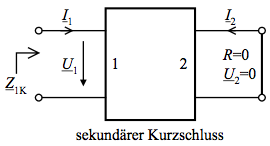
\includegraphics[height=1.8cm]{./bilder/sekKurzschluss}\\
			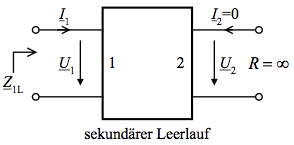
\includegraphics[height=1.8cm]{./bilder/sekLeerlauf}
	    \end{minipage}
		\begin{minipage}{4cm}
	    	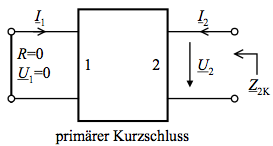
\includegraphics[height=1.8cm]{./bilder/primKurzschluss}\\
			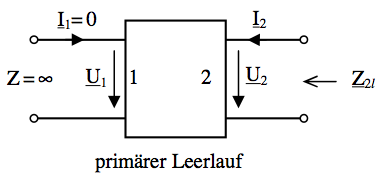
\includegraphics[height=1.8cm]{./bilder/primLeerlauf}
	    \end{minipage}

% 
% \subsection{Eingangsimpedanz und Übertragungsgrössen bei beliebiger Last}
% 	\renewcommand{\arraystretch}{1.1}
% 		\begin{tabular}{| c | c | c | c | c | c |}
% 			\hline
% 				\textbf{Bezeichnung}
% 				& \textbf{Definition} 
% 				& \textbf{Berechnung} 
% 				& \textbf{}
% 				& \textbf{Quelle}
% 				& \textbf{Betriebsrichtung}\\
% 			\hline
% 				\textbf{$\underline{Z}_{1}$}
% 				& $ \frac{\underline{U}_{1}}{\underline{I}_{1}}=$
% 				& $ \frac{\underline{A}_{11}\underline{Z}_{b}+\underline{A}_{12}}{\underline{A}_{21}\underline{Z}_{b}+\underline{A}_{22}}=$
% 				& $ \frac{\underline{Z}_{11}\underline{Z}_{b}+\det(Z)}{\underline{Z}_{b}+\underline{Z}_{22}}$
% 				& $ \underline{I}_{1}$
% 				& vorwärts\\
% 			\hline
% 				\textbf{$\underline{Z}_{2}$}
% 				& $ \frac{\underline{U}_{2}}{\underline{I}_{2}}=$
% 				& $ \frac{\underline{A}_{22}\underline{Z}_{a}+\underline{A}_{12}}{\underline{A}_{21}\underline{Z}_{a}+\underline{A}_{11}}=$
% 				& $ \frac{\underline{Z}_{22}\underline{Z}_{a}+\det(Z)}{\underline{Z}_{a}+\underline{Z}_{11}}$
% 				& $ \underline{I}_{2}$
% 				& rückwärts\\
% 			\hline
% 				\textbf{$\underline{Z}_{ba}$}
% 				& $ \frac{\underline{U}_{2}}{\underline{I}_{1}}=$
% 				& $ \frac{\underline{b}_{b}}{\underline{A}_{21}\underline{b}_{b}+\underline{A}_{22}}=$
% 				& $ \frac{\underline{Z}_{21}\underline{Z}_{b}}{\underline{Z}_{b}+\underline{Z}_{22}}$
% 				& $ \underline{I}_{1}$
% 				& vorwärts\\
% 			\hline
% 				\textbf{$\underline{Z}_{ab}$}
% 				& $ \frac{\underline{U}_{1}}{\underline{I}_{2}}=$
% 				& $ \frac{\underline{Z}_{a}\cdot \det(A)}{\underline{A}_{21}\underline{Z}_{b}+\underline{A}_{22}}=$
% 				& $ \frac{\underline{Z}_{12}\underline{Z}_{a}}{\underline{Z}_{a}+\underline{Z}_{11}}$
% 				& $ \underline{I}_{2}$
% 				& rückwärts\\
% 			\hline
% 				\textbf{$\underline{Y}_{ba}$}
% 				& $ \frac{\underline{I}_{2}}{\underline{U}_{1}}=$
% 				& $ \frac{-1}{\underline{A}_{11}\underline{Z}_{a}+\underline{A}_{12}}=$
% 				& $ \frac{-\underline{Z}_{21}}{\underline{Z}_{11}\underline{Z}_{b}+\det(Z)}$
% 				& $ \underline{U}_{1}$
% 				& vorwärts\\
% 			\hline
% 				\textbf{$\underline{Y}_{ab}$}
% 				& $ \frac{\underline{U}_{1}}{\underline{I}_{2}}=$
% 				& $ \frac{-\det(A)}{\underline{A}_{22}\underline{Z}_{a}+\underline{A}_{12}}=$
% 				& $ \frac{-\underline{Z}_{12}}{\underline{Z}_{22}\underline{Z}_{a}+\det(Z)}$
% 				& $ \underline{U}_{2}$
% 				& rückwärts\\
% 			\hline
% 		\end{tabular}
% 	\renewcommand{\arraystretch}{1}
% 		\begin{minipage}{5cm}
% 	    	Vorwärts:\\
% 			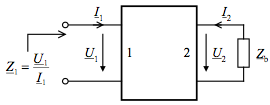
\includegraphics[height=1.8cm]{./bilder/vorwaertsEingangsimpedanz}\\
% 			Rückwärts:\\
% 			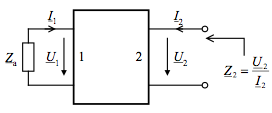
\includegraphics[height=1.8cm]{./bilder/rueckwaertsEingangsimpedanz}
% 	    \end{minipage}	
% \\\textcolor{red}{Die Spannungs und Stromübersetzung T brauchts nicht, oder?}


\subsection{Zusammenschalten von 2-Toren}
\begin{tabular}{|l|l|l|l|}
\hline
 Serieschaltung & Serie-Parallelschaltung & Parallelschaltung & Kettenschaltung\\
\hline
\begin{tikzpicture}[scale=0.8]
	\draw (0,0) -- (1,0);
	\draw (0,3) -- (1,3);
	\draw (1,0) -- (1.5,0);
	\draw (1,1) -- (1.5,1);
	\draw (1,1) -- (1,2);
	\draw (1,3) -- (1.5,3);
	\draw (1,2) -- (1.5,2);
	\draw (1.5,-0.2) rectangle (3,1.2);
	\draw (1.5,1.8) rectangle (3,3.2);
	\node at (2.25,0.5) {$[Z'']$};
	\node at (2.25,2.5) {$[Z']$};
	\draw (3,0) -- (3.5,0);
	\draw (3,1) -- (3.5,1);
	\draw (3.5,1) -- (3.5,2);
	\draw (3,2) -- (3.5,2);
	\draw (3,3) -- (3.5,3);
	\draw (3.5,3) -- (4.5,3);
	\draw (3.5,0) -- (4.5,0);
	\draw [dashed] (0.5,-0.5) rectangle (4,3.5);
\end{tikzpicture}&
\begin{tikzpicture}[scale=0.8]
	\draw (0,0) -- (1,0);
	\draw (0,3) -- (1,3);
	\draw (1,0) -- (1.5,0);
	\draw (1,1) -- (1.5,1);
	\draw (1,1) -- (1,2);
	\draw (1,3) -- (1.5,3);
	\draw (1,2) -- (1.5,2);
	\draw (1.5,-0.2) rectangle (3,1.2);
	\draw (1.5,1.8) rectangle (3,3.2);
	\node at (2.25,0.5) {$[H'']$};
	\node at (2.25,2.5) {$[H']$};
	\node at (2.25,1.45) {$[H]$};
	\draw (3,0) -- (3.5,1);
	\draw (3,1) -- (3.5,2);
	\draw (3,2) -- (3.5,1);
	\draw (3,3) -- (3.5,2);
	\draw (3.5,1) -- (4.5,1);
	\draw (3.5,2) -- (4.5,2);
	\draw [dashed] (0.5,-0.5) rectangle (4,3.5);
\end{tikzpicture}&
\begin{tikzpicture}[scale=0.8]
	\draw (0,1) -- (1,1);
	\draw (0,2) -- (1,2);
	\draw (1,1) -- (1.5,0);
	\draw (1,2) -- (1.5,1);
	\draw (1,2) -- (1.5,3);
	\draw (1,1) -- (1.5,2);
	\draw (1.5,-0.2) rectangle (3,1.2);
	\draw (1.5,1.8) rectangle (3,3.2);
	\node at (2.25,0.5) {$[Y'']$};
	\node at (2.25,2.5) {$[Y']$};
	\node at (2.25,1.45) {$[Y]$};
	\draw (3,0) -- (3.5,1);
	\draw (3,1) -- (3.5,2);
	\draw (3,2) -- (3.5,1);
	\draw (3,3) -- (3.5,2);
	\draw (3.5,1) -- (4.5,1);
	\draw (3.5,2) -- (4.5,2);
	\draw [dashed] (0.5,-0.5) rectangle (4,3.5);
\end{tikzpicture}&
\begin{tikzpicture}[scale=0.8]
	\draw (0,0) -- (1,0);
	\draw (0,1) -- (1,1);
	\draw (1,-0.2) rectangle (2.5,1.2);
	\node at (1.75,0.5) {$[A']$};
	\draw (2.5,0) -- (3.5,0);
	\draw (2.5,1) -- (3.5,1);
	\draw (3.5,-0.2) rectangle (5,1.2);
	\node at (4.25,0.5) {$[A'']$};
	\draw (5,0) -- (6,0);
	\draw (5,1) -- (6,1);
	\draw [dashed] (0.5,-0.5) rectangle (5.5,1.5);
	\node at (3,-0.25) {$[A]$};
\end{tikzpicture}\\
\hline
\end{tabular}\\
	\renewcommand{\arraystretch}{1.1}
		\begin{tabular}{| c | c | c |}
			\hline
				\textbf{Schaltung}
				& \textbf{Matrix} 
				& \textbf{allgemeine Form}\\
			\hline
				\textbf{Serieschaltung}
				& $ [Z]=[Z']+[Z'']$
				& $ \begin{matrix}
						\underline{U}_{1}=(\underline{Z'}_{11}+\underline{Z''}_{11})\underline{I}_{1}+(\underline{Z'}_{12}+\underline{Z''}_{12})\underline{I}_{2}\\
						\underline{U}_{2}=(\underline{Z'}_{21}+\underline{Z''}_{21})\underline{I}_{1}+(\underline{Z'}_{22}+\underline{Z''}_{22})\underline{I}_{2}\\
					\end{matrix}$\\
			\hline
				\textbf{Parallelschaltung}
				& $ [Y]=[Y']+[Y'']$
				& $ \begin{matrix}
						\underline{I}_{1}=(\underline{Y'}_{11}+\underline{Y''}_{11})\underline{U}_{1}+(\underline{Y'}_{12}+\underline{Y''}_{12})\underline{U}_{2}\\
						\underline{I}_{2}=(\underline{Y'}_{21}+\underline{Y''}_{21})\underline{U}_{1}+(\underline{Y'}_{22}+\underline{Y''}_{22})\underline{U}_{2}\\
					\end{matrix}$\\
			\hline
				
				$ \begin{matrix}
					\textbf{Serie-}\\
					\textbf{Parallelschaltung}
				  \end{matrix}$
				& $ [H]=[H']+[H'']$
				& $ \begin{matrix}
						\underline{U}_{1}=(\underline{H'}_{11}+\underline{H''}_{11})\underline{I}_{1}+(\underline{H'}_{12}+\underline{H''}_{12})\underline{U}_{2}\\
						\underline{I}_{2}=(\underline{H'}_{21}+\underline{H''}_{21})\underline{I}_{1}+(\underline{H'}_{22}+\underline{H''}_{22})\underline{U}_{2}\\
					\end{matrix}$\\
			\hline
				\textbf{Kettenschaltung}
				& $ [A]=[A']\cdot[A'']$
				& $ \begin{matrix}
						\underline{U}_{1}=(\underline{A'}_{11}\underline{A''}_{11}+\underline{A'}_{12}\underline{A''}_{21})\underline{U}_{2}+(\underline{A'}_{11}\underline{A''}_{12}+\underline{A'}_{12}\underline{A''}_{22})\underline{I}_{2}\\
						\underline{I}_{1}=(\underline{A'}_{21}\underline{A''}_{11}+\underline{A'}_{22}\underline{A''}_{21})\underline{U}_{2}+(\underline{A'}_{21}\underline{A''}_{12}+\underline{A'}_{22}\underline{A''}_{22})\underline{I}_{2}\\
					\end{matrix}$\\
			\hline
		\end{tabular}
	\renewcommand{\arraystretch}{\arraystretchOriginal}
\subsection{Umkehrung eines 2-Tores}
	\renewcommand{\arraystretch}{1.1}
		\begin{tabular}{| c | c | c |}
			\hline
				\textbf{}
				& \textbf{$\tilde{X}$}
				& \textbf{$\det(\tilde{X})$}\\
			\hline
				\textbf{$\tilde{Z}$}
				& $\begin{bmatrix}
						\underline{Z}_{22} & \underline{Z}_{21} \\
						\underline{Z}_{12} & \underline{Z}_{11} \\
					\end{bmatrix}$
				& $\det(Z)$\\
			\hline
				\textbf{$\tilde{Y}$}
				& $\begin{bmatrix}
						\underline{Y}_{22} & \underline{Y}_{21} \\
						\underline{Y}_{12} & \underline{Y}_{11} \\
					\end{bmatrix}$
				& $\det(Y)$\\
			\hline
				\textbf{$\tilde{A}$}
				& $\frac{1}{\det(A)} 
					\begin{bmatrix}
						\underline{A}_{22} & \underline{A}_{12} \\
						\underline{A}_{21} & \underline{A}_{11} \\
					\end{bmatrix}$
				& $\frac{1}{der(A)}$\\
			\hline
				\textbf{$\tilde{H}$}
				& $\frac{1}{\det(H)} 
					\begin{bmatrix}
						\underline{H}_{11} & -\underline{H}_{21} \\
						-\underline{H}_{12} & \underline{H}_{22} \\
					\end{bmatrix}$
				& $\frac{1}{\det(H)}$\\
			\hline
		\end{tabular}
	\renewcommand{\arraystretch}{\arraystretchOriginal}
	
	
	

		
\newpage


\section{Leitungstheorie}

\subsection{Leitungsgleichungen}
	\begin{tabular}{p{8cm}p{4.5cm}p{5cm}}
		\begin{minipage}{8cm}
	    	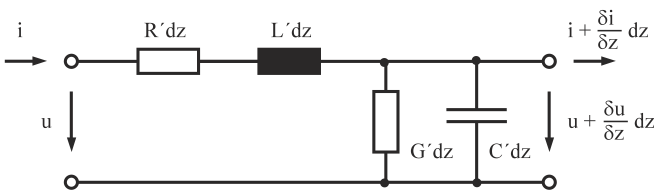
\includegraphics[width=8cm]{/bilder/LeitungselementESB.png}
	    \end{minipage}&
		\begin{minipage}{4.5cm}
	    	\textbf{Leitungsbeläge}\\
	    	$R'[\frac{\Omega}{m}]: \text{Widerstandsbelag}$\\
	    	$L'[\frac{H}{m}]: \text{Induktivitätsbelag}$\\
	    	$G'[\frac{S}{m}]: \text{Leitwertbelag}$\\
	    	$C'[\frac{F}{m}]: \text{Kapazitätsbelag}$\\
	    \end{minipage}&
		\begin{minipage}{5cm}
        	\textbf{Leerlauf}:\\
        		$\underline{Y}_L=\frac{1}{\underline{Z}_L}=\frac{\underline{I}_L}
        		{U} = G+j\omega C=\frac{\alpha l+j\beta l}{\underline{Z}_W}$\\
        	\textbf{Kurzschluss}:\\
        		$\underline{Z_K}=\frac{U}{\underline{I}_K} = R+j\omega
        		L=(\alpha l+j\beta l)\underline{Z}_W$\\
        \end{minipage}\\
		\begin{minipage}{8cm}
        	\vspace{0.3cm}
        	$\underline{U}_1=\cosh(\gamma l)\cdot \underline{U}_2+
        	\underline{Z}_W \cdot \sinh(\gamma l)\cdot \underline{I}_2$\\
  			$\underline{I}_1=\frac{1}{\underline{Z}_W}\cdot \sinh(\gamma l)\cdot
  			\underline{U}_2+ \cosh(\gamma l)\cdot \underline{I}_2$  	
        \end{minipage} &
		\begin{minipage}{9cm}
        \vspace{0.3cm}
		$\begin{bmatrix}
          	\underline{U}_1\\
          	\underline{I}_1
          \end{bmatrix}=
		  \begin{bmatrix}
          	cosh(\gamma l) & \underline{Z}_W sinh(\gamma l)\\
          	\frac{1}{\underline{Z}_W}sinh(\gamma l) & cosh(\gamma l)
          \end{bmatrix} \cdot
		  \begin{bmatrix}
          	\underline{U}_2\\
          	\underline{I}_2
          \end{bmatrix}$\\
        \end{minipage}
	\end{tabular}\\
		wenn $\alpha l >> \beta l$ kann $cosh(\gamma l)\approx sinh(\gamma
		l)=\frac{1}{2} e^{\gamma l}$ angenommen werden!!!
	

	\subsubsection{Verlustbehaftete Leitungen}
		\renewcommand{\arraystretch}{1.5}
		\begin{tabular}{| p{7.7cm} | l |}
			\hline
				\textbf{Fortpflanzungskonstante}
				& $\gamma=\alpha+j\beta=\sqrt{(R'+j\omega L')(G'+j\omega C')}\qquad
				\alpha=[\frac{Np}{m}] \qquad \beta=[\frac{^\circ}{m}]$\\
			\hline
				\textbf{Dämpfungsmass}
				& $\alpha l= \frac{1}{2}ln(Re\{e^{2\gamma l}\})=\alpha\cdot l$\\
			\hline
				\textbf{Phasenmass}
				& $\beta l=\frac{1}{2}ln(Im\{e^{2\gamma l}\})= \beta\cdot l$ \qquad
				$\beta=\frac{\omega}{v_P}$\\
			\hline
				\textbf{Wellenwiderstand}
				& $\underline{Z}_W=\frac{\underline{U}}{\underline{I}}=\sqrt{\frac{R'+j\omega L'}{G'+j\omega C'}}$
				$=\sqrt{\underline{Z}_L \cdot \underline{Z}_K}$\\
			\hline
				\textbf{Eingangswid. $\underline{Z}_1$  bei Abschluss mit
				Lastwid. $\underline{Z}_a$} &
				$\underline{Z}_1 = \underline{Z}_W
				\frac{\underline{Z}_a+\underline{Z}_W \cdot \tanh(\gamma
				l)}{\underline{Z}_W+\underline{Z}_a \cdot \tanh(\gamma l)}
				= \underline{Z}_W \frac{e^{+j \gamma l} + \underline{\Gamma}_{Last} e^{- j \gamma l}}
				{e^{+j \gamma l} - \underline{\Gamma}_{Last} e^{- j \gamma l}}$\\
			\hline
				\textbf{Phasengeschwindigkeit, Wellenlänge}
				& $v_P=\frac{1}{\sqrt{L'C'}}=\frac{\lambda}{T}$ \qquad
				\qquad $\lambda=\frac{2\pi}{\beta}=\frac{v_P}{f} \approx
				\lambda=\frac{\lambda_0}{\sqrt{\varepsilon_r \mu_r}} \quad \beta=[rad]$\\
			\hline
				\textbf{Freiraumwellenlänge}
				& $\lambda_0=\frac{c}{f}=\frac{2\pi c}{\omega} \qquad c\approx 3*10^8 \frac{m}{s}$\\
			\hline
				\textbf{Wellengleichung}
				& $\begin{matrix}
                   	\underline{U}(z)=\underline{U}^+_0 \cdot e^{-\gamma z} + \underline{U}^-_0 \cdot e^{\gamma z}\\
                   	\underline{I}(z)=\underline{I}^+_0 \cdot e^{-\gamma z} - \underline{U}^-_0 \cdot e^{\gamma z}\\
                   	\qquad \text{\tiny hinlaufend}\qquad\text{\tiny rücklaufend}
                \end{matrix}$\\
			\hline
				\textbf{Reflektions-, Transmissionskoeffizienten}
				&
				$\underline{\Gamma}_{Last}=\frac{\underline{U}^-}{\underline{U}^+}=\frac{\underline{Z}_{Last}-\underline{Z}_W}
				{\underline{Z}_{Last}+\underline{Z}_W}$ \quad bzw. \quad
				$\underline{\Gamma}_{Quelle}=\frac{\underline{Z}_{Quelle}-\underline{Z}_W}
				{\underline{Z}_{Quelle}+\underline{Z}_W}$
				\qquad $\underline{\tau} = 1 + \underline{\Gamma}$\\
			\hline
				\textbf{Keine Reflektion bei:}
				& $\underline{Z}_{Last}=\underline{Z}_W$ \quad bzw.
				\quad $\underline{Z}_{Quelle}=\underline{Z}_W$\\
			\hline
				\textbf{Totalreflexion}
				& $\begin{matrix}
					\underline{\Gamma}=-1 \Rightarrow \underline{Z}_{Last}=\underline{Z}_{Quelle}=0 \quad
					\text{ideale U-Quelle (Kurzschluss)}\\
					\underline{\Gamma}=+1 \Rightarrow \underline{Z}_{Last}=\underline{Z}_{Quelle}=\infty \qquad
					\text{ideale I-Quelle (Leerlauf)} \end{matrix}$\\
			\hline
				\textbf{Neper}
				& $1 dB=\frac{ln(10)}{20}Np$ \qquad $U_2 = U_1 \cdot e^{L_U}$\\
			\hline
				\textbf{Bei Abschluss mit $\underline{Z}_W$} &
				$\underline{U}_1(z) = \underline{U}_2\cdot e^{\gamma z} \qquad
				\underline{I}_1(z) =- \underline{I}_2\cdot e^{\gamma z} \qquad \alpha l =
				ln(\frac{U1}{U2}) \qquad \beta l = arg(\frac{\underline{U}_1}{\underline{U}_2})$\\
			\hline
				\textbf{wichtige Formeln}&
				$\gamma l=\frac{1}{2}ln(\frac{1+\sqrt{\underline{Z}_K/\underline{Z}_L}}{1-
				\sqrt{\underline{Z}_K/\underline{Z}_L}})$ \qquad
				$\sqrt{\frac{\underline{Z}_K}{\underline{Z}_L}}=\frac{e^{2\gamma
				L}-1}{e^{2\gamma K}+1}$ \qquad $e^{2\gamma l}=e^{2\alpha l} \cdot e^{j2\beta
				l}=\frac{1+\sqrt{{\underline{Z}_K}/
				{\underline{Z}_L}}}{1-\sqrt{{\underline{Z}_K}/ {\underline{Z}_L}}}$\\
			\hline
		\end{tabular}
	\renewcommand{\arraystretch}{1}
	
	
	\subsubsection{Verlustfreie Leitungen}
		\renewcommand{\arraystretch}{1.5}
		\begin{tabular}{| l | c |}
			\hline
				\textbf{Fortpflanzungskonstante}
				& $\gamma=j\beta=j\omega \sqrt{L'C'} \qquad R'=G'=\alpha=0$\\
			\hline
				\textbf{Dämpfungsmass}
				& $\alpha=0$\\
			\hline
				\textbf{Phasenmass}
				& $\beta=\frac{2\pi}{\lambda}=\omega\sqrt{L'C'}$\\
			\hline
				\textbf{Wellenwiderstand}
				& $Z_W=\sqrt{\frac{L'}{C'}}$\\
			\hline
				\textbf{LE Leerlauf} $\underline{I}_2=0 \quad \underline{\Gamma}=1$
				& $\underline{Z}_1=-j\frac{\underline{Z}_W}{\tan(\beta l)}$\\
			\hline
				\textbf{LE Kurzschluss} $\underline{U}_2=0 \quad \underline{\Gamma}=-1$
				& $\underline{Z}_1=j \underline{Z}_W \tan(\beta l)$\\
			\hline
				$\begin{matrix}
					\textbf{LE mit }\underline{Z}_{Last} \textbf{ abgeschlossen}\\
					%\underline{Z}_L=\underline{Z}_W \quad \underline{\Gamma}=0
				\end{matrix}$
				& $\begin{matrix}
                  	\frac{\underline{U}_1}{\underline{I}_2}=\cosh(j\beta
                  	l)\underline{Z}_{Last}+\underline{Z}_W \sinh(j\beta l)\\
                  	\frac{\underline{I}_1}{\underline{I}_2}=\frac{1}{\underline{Z}_W} \sinh(j\beta
                  	l)\underline{Z}_{Last}+ \cosh(j\beta l) \end{matrix}$\\
			\hline
		\end{tabular}
	\renewcommand{\arraystretch}{1}
	\newpage
% 	\subsubsection{Leitungen in Vierpolnotation}
% 	\renewcommand{\arraystretch}{1.1}
% 		\begin{tabular}{| l | c |}
% 			\hline
% 				\textbf{A Matrix}
% 				& $\begin{bmatrix}
%                   	\underline{U}_1\\
%                   	\underline{I}_1
%                   \end{bmatrix}=
% 				  \begin{bmatrix}
%                   	cosh(\gamma l) & \underline{Z}_W sinh(\gamma l)\\
%                   	\frac{1}{\underline{Z}_W}sinh(\gamma l) & cosh(\gamma l)
%                   \end{bmatrix} \cdot
% 				  \begin{bmatrix}
%                   	\underline{U}_2\\
%                   	\underline{I}_2
%                   \end{bmatrix}$\\
% 			\hline
% 				\textbf{T-Ersatz}
% 				& $\underline{Z}_1=tanh(\frac{\gamma l}{2})\underline{Z}_W=\underline{Z}_2$\\
% 			\hline
% 				\textbf{Pi-Ersatz}
% 				& $\underline{Z}_1=\frac{\underline{Z}_W}{tanh(\frac{\gamma l}{2})}=\underline{Z}_2$\\
% 			\hline
% 		\end{tabular}
% 	\renewcommand{\arraystretch}{1}


\subsection{Kapazitätsbelag}
	\begin{tabular}{ll}
    	\begin{minipage}{12cm}
			\renewcommand{\arraystretch}{1.1}
				\begin{tabular}{| l | l |}
					\hline
						\textbf{Leiterpotential}
						& $\vec{E}=-grad V$ \qquad $V(\varrho)=-\frac{\lambda}{\varepsilon_02\pi}ln\frac{\varrho}{k}$\\
					\hline
						\textbf{$\varrho$}
						& $\begin{matrix}
                           		\text{Abstand zwischen Linienladungen}\\
                           		\text{und deren Spiegelungen}
                           \end{matrix}$\\
					\hline
						\textbf{$k$}
						& Integrationskonstante (kürzt sich weg)\\
					\hline
						\textbf{$\varepsilon_0$}
						& $8,85419 \cdot 10^{-12} [\frac{As}{Vs}]$\\
					\hline
						$\begin{matrix}
                         	\textbf{Leiterpotentiale}\\
                         	(aus Beispiel)
                         \end{matrix}$
						& $\begin{matrix}
                          	V_1=\frac{\lambda_1}{2\pi\varepsilon_0}(-ln\frac{r}{k}+ln\frac{2a}{k})+\frac{\lambda_2}{2\pi\varepsilon_0}(-ln\frac{\varrho_1}{k}+ln\frac{\varrho_2}{k})\\
                          	V_2=\frac{\lambda_1}{2\pi\varepsilon_0}(-ln\frac{\varrho_1}{k}+ln\frac{\varrho_2}{k})+\frac{\lambda_2}{2\pi\varepsilon_0}(-ln\frac{r}{k}+ln\frac{2b}{k})
                          \end{matrix}$\\
					\hline
						\textbf{Matrix Potentialkoeff.}
						& $ \begin{bmatrix}
								V_1 \\
								V_2 \\
							\end{bmatrix}=
							\begin{bmatrix}
								p_1 & p_0 \\
								p_0 & p_2 \\
							\end{bmatrix} \cdot
							\begin{bmatrix}
								\lambda_1 \\
								\lambda_2 \\
							\end{bmatrix}$\\
					%\hline
						\textbf{}
						& $p_1=\frac{1}{2\pi \varepsilon_0}ln\frac{2a}{r}$ \quad
						  $p_2=\frac{1}{2\pi \varepsilon_0}ln\frac{2b}{r}$ \quad
				          $p_0=\frac{1}{2\pi \varepsilon_0}ln\frac{\varrho_1}{\varrho_2}$\\
					\hline
						\textbf{Matrix Kapazitätskoeff.}
						& $ \begin{bmatrix}
								\lambda_1 \\
								\lambda_2 \\
							\end{bmatrix}=
							\begin{bmatrix}
								C_1 & C_0 \\
								C_0 & C_2 \\
							\end{bmatrix} \cdot
							\begin{bmatrix}
								V_1 \\
								V_2 \\
							\end{bmatrix}$\\
					%\hline
						\textbf{}
						& $C_1=\frac{p_2}{det\quad p}$ \quad
						  $C_2=\frac{p_1}{det\quad p}$ \quad
						  $C_0=\frac{p_0}{det\quad p}=C_{12}$\\
						  &$C_{10}=C_1-C_0; C_{20}=C_2-C_0$\\
					\hline
				\end{tabular}
			\renewcommand{\arraystretch}{1}
		\end{minipage}
    \end{tabular}
	\begin{minipage}{6cm}
    	\begin{tabular}{ll}
	    	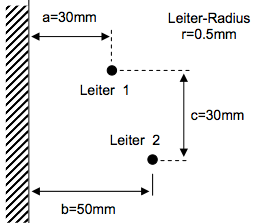
\includegraphics[width=3cm]{../El4/bilder/LeitungenParallel.png}
			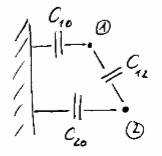
\includegraphics[width=3cm]{../El4/bilder/LeitungenKapazitaeten.png} \\
			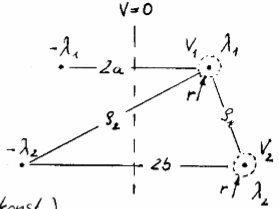
\includegraphics[width=5cm]{../El4/bilder/LeitungenParallel2.png}
		\end{tabular}
	\end{minipage}
 
		
\subsection{Induktivitätsbelag}
	\begin{tabular}{ll}
    	\begin{minipage}{12cm}
			\renewcommand{\arraystretch}{1.1}
				\begin{tabular}{| l | l |}
					\hline
						\textbf{Rotation B-Feld}
						& $\vec{B}=rot\vec{A}$ \qquad $A(\varrho)=-\frac{\mu_0 I}{2\pi}ln(\frac{\varrho}{k})$\\
					\hline
						\textbf{Linienströme}
						& $+I \qquad -I$\\
					\hline
						\textbf{$\mu_0$}
						& $4\pi\cdot 10^{-7}[\frac{Vs}{Am}]$\\
					\hline
						$\begin{matrix}
                         	\textbf{Leiterpotentiale}\\
                         	(aus Beispiel)
                         \end{matrix}$
						& $\begin{matrix}
                           	A^{+}=\frac{\mu_0 I}{2\pi}(-ln\frac{r}{k}+ln\frac{\varrho_1}{k}-ln\frac{2a}{k}+ln\frac{\varrho_2}{k})=\frac{\mu_0 I}{2\pi}ln\frac{\varrho_1\varrho_2}{2ar}\\
                           	A^{-}=\frac{\mu_0 I}{2\pi}(-ln\frac{\varrho_1}{k}+ln\frac{r}{k}-ln\frac{\varrho_2}{k}+ln\frac{2b}{k})=-\frac{\mu_0 I}{2\pi}ln\frac{\varrho_1\varrho_2}{2br}
                           \end{matrix}$\\
					\hline
						\textbf{Äussere Induktivität}
						& $L_a=\frac{1}{I}(A^{+}-A^{-})=\frac{\mu_0}{2\pi}ln(\frac{\varrho_1^2 \varrho_2^2}{4r^2ab})$\\
					\hline
						\textbf{Innere Induktivität}
						& $L_i=\frac{\mu_0}{8\pi} \quad \text{pro Leiter}$\\
					\hline
						\textbf{Induktivitätsbelag}
						& $L'=L_a+2L_i=\frac{\mu_0}{\pi} (ln(\frac{\varrho_1 \varrho_2}{2r\sqrt{ab}})+\frac{1}{4})$\\
					\hline
				\end{tabular}
			\renewcommand{\arraystretch}{1}
		\end{minipage}
    \end{tabular}
	\begin{minipage}{6cm}
    	\begin{tabular}{ll}
	    	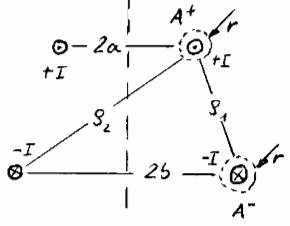
\includegraphics[width=5cm]{../El4/bilder/Induktivitaetsbelag.png}
		\end{tabular}
	\end{minipage}

\subsection{Stehende Wellen}
%	\subsubsection{Eigenschaften}
		\begin{tabular}{ll}
	    	\begin{minipage}{9cm}
				\renewcommand{\arraystretch}{1.1}
					\begin{tabular}{| l | l |}
						\hline
							\textbf{Spannung}
							& $|\underline{U}(z)|=|\underline{U}^+ e^{-j\beta z}(1+\underline{\Gamma}_L e^{2j\beta z})|=|\underline{U}^+| |1+\underline{\Gamma}_L e^{2j\beta z}|=|\underline{U}^+||1+|\underline{\Gamma}_L| e^{j(\Phi-2\beta z)}|$\\
						\hline
							\textbf{Strom}
							& $|\underline{I}(z)|=|\underline{U}^+ / \underline{Z}||1-|\underline{\Gamma}_L| e^{j(\Phi-2\beta z)}|$\\
						\hline
							\textbf{Spannungsmaxima bei:}
							& $e^{j(\Phi-2\beta z)}=1$\\
						\hline
							\textbf{Spannungsminima bei:}
							& $e^{j(\Phi-2\beta z)}=-1$\\
						\hline
					\end{tabular}
				\renewcommand{\arraystretch}{1}
			\end{minipage}
	    \end{tabular}

		\begin{tabular}{p{9cm}p{9cm}}
        	\begin{minipage}{8cm}
            	Spannungsbetrag mit kompl. Abschlussimpedanz:\\
            	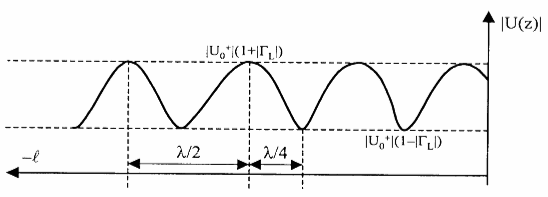
\includegraphics[height=2cm]{../El4/bilder/VerlaufSpannungsbetrag.png}
            \end{minipage}
			&
			\begin{minipage}{8cm}
            	Spannungs- Strombetrag der offenen Leitung:\\
            	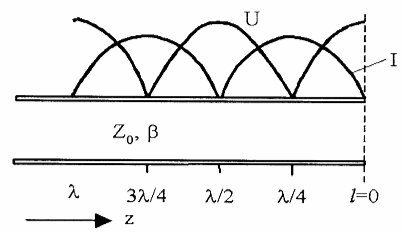
\includegraphics[height=2cm]{../El4/bilder/VerlaufSpannungsbetragOffeneLtg.png}
            \end{minipage}
        \end{tabular}
	
	\subsubsection{Spezialfälle}
		\textbf{Kurzschluss/Leerlauf}\\
			Bei Kurzschluss oder Leerlauf, also Reflexionsfaktor $\underline{\Gamma}$ ist -1 oder 1, verschwinden die Spannungs- Stromminima.
			Da die rückläufige Welle ebensoviel Energie transportiert wie die hinlaufende, wird längs der Leitung keine Energie transportiert.
			Es sieht also so aus, als ob die Welle am Ort stehen bleibt (Bild 2).\\
		\textbf{Leitung ideal abgeschlossen}\\
			Ist die Leitung ideal abgeschlossen, existiert keine reflektierende Welle.
			Die hinlaufende Welle transportiert so die gesammte Energie vom Sender zum Empfänger.\\
		\textbf{Leitung nicht ideal abgeschlossen}\\
			Es entsteht beim Empfänger eine Überlagerung der absorbierten und der stehenden Welle.
			Aus dem Verhältnis von Spannungsmaximum zu Spannungsminimum entsteht das Stehwellenverhältnis SWR.
			
			$$\text{Stehwellenverhältnis}: \quad SWR=\frac{U_{max}}{U_{min}}=\frac{1+|\Gamma_L|}{1-|\Gamma_L|} \qquad \text{Betrag des Reflexionsfaktor}:|\Gamma_L|=\frac{\text{SWR} -1}{\text{SWR} +1}$$

	\subsection{Mehrfachreflexion}
% 	\textbf{Lastseitig falsch abgeschlossen}\\
% 	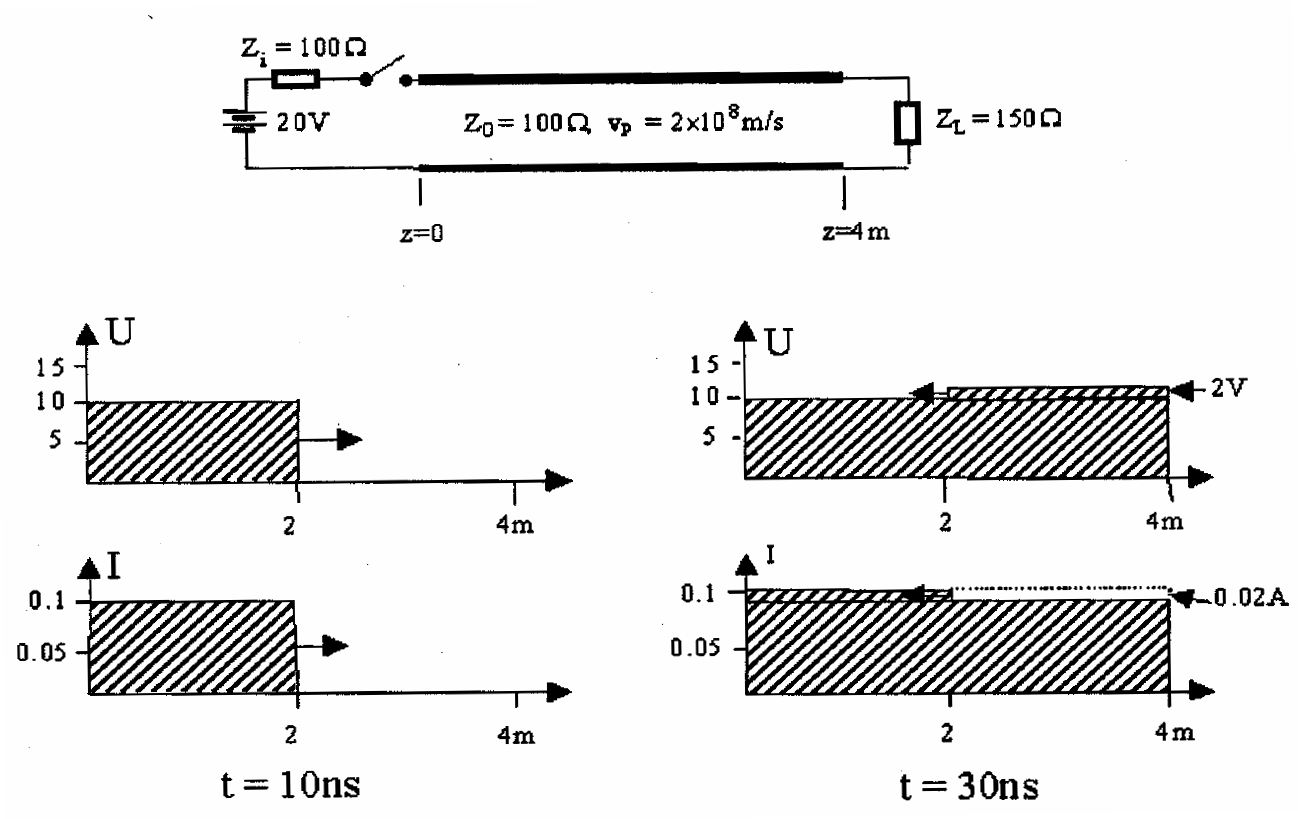
\includegraphics[height=3.5cm]{../El4/bilder/Leitungen_MFReflx_EnAP_SAP.png} \textbf{text folgt} \\
	\begin{tabular}{p{9cm}p{9cm}}
		\begin{minipage}{8cm}
			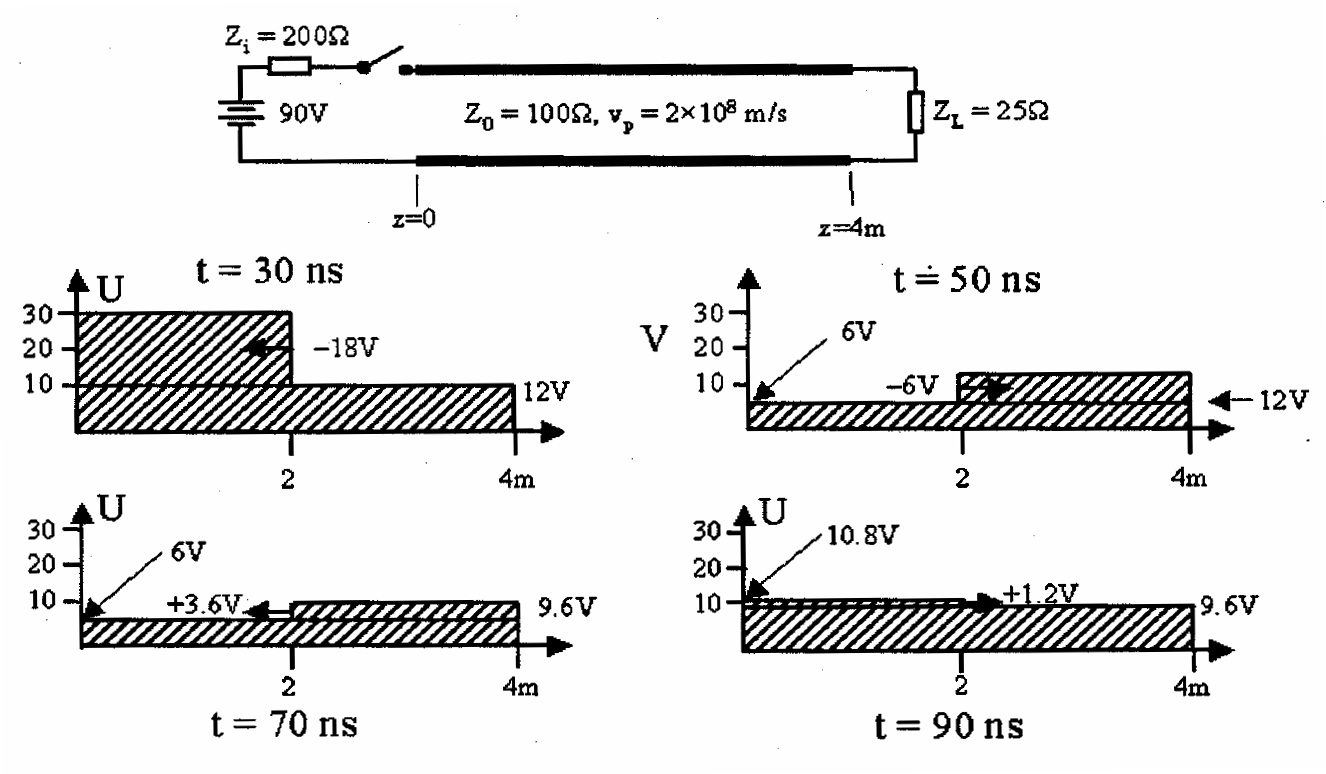
\includegraphics[width=8cm]{../El4/bilder/Leitungen_MFReflx_EnAP_SnAP.png}
	    \end{minipage}
		&
		\begin{minipage}{9cm} 	    	
    		Das nebenstehende Schema zeigt eine Leitung, welche last- und quellenseitig falsch
    		abgeschlossen ist. \\
    		Zur Berechnung der Spannung $\underline{U}_{0}^+$ werden alle Widerstände am Leitungsende
    		ignoriert ($\underline{Z}_L = 0$).
    		Die reflektierenden Wellen werden anhand der Reflexionskoeffizienten
    		$\underline{\Gamma}_{Last}, \underline{\Gamma}_{Quelle}$ berechnet. Bsp.:
    		\\ \\
    		$\underline{U}_{0}^+ = \frac{U_{Quelle} \underline{Z}_0}{ \underline{Z}_0 +
    		\underline{Z}_i}; \quad \underline{U}_{0}^- = \underline{U}_{0}^+ \cdot 
    		\underline{\Gamma}_{Last}; \\ \underline{U}_{1}^+ = \underline{U}_{0}^- \cdot 
    		\underline{\Gamma}_{Quelle}; \quad
    		\underline{U}_{1}^- = \underline{U}_{1}^+ \cdot 
    		\underline{\Gamma}_{Last}; \quad$ usw.   \\ 
    		$\underline{U}_{Resultierend} = \underline{U}_{0}^+ + \underline{U}_{0}^- +
    		\underline{U}_{1}^+ + \underline{U}_{1}^- +  \ldots  + \underline{U}_{n}^+ +
    		\underline{U}_{n}^-$
	    \end{minipage}  
		\\
		\begin{minipage}{8cm}  
			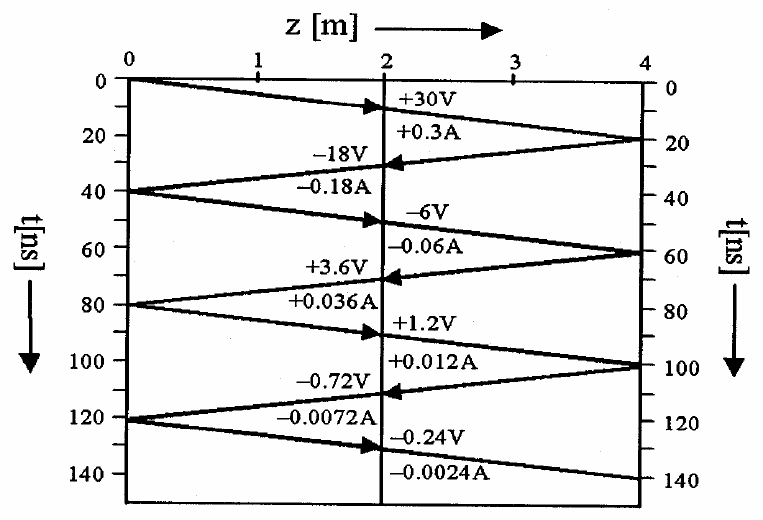
\includegraphics[height=4.1cm]{../El4/bilder/Leitungen_MFReflx_EnAP_SnAP_RaumZeit.png}    	    
	    \end{minipage}
		&
		\begin{minipage}{8cm}
			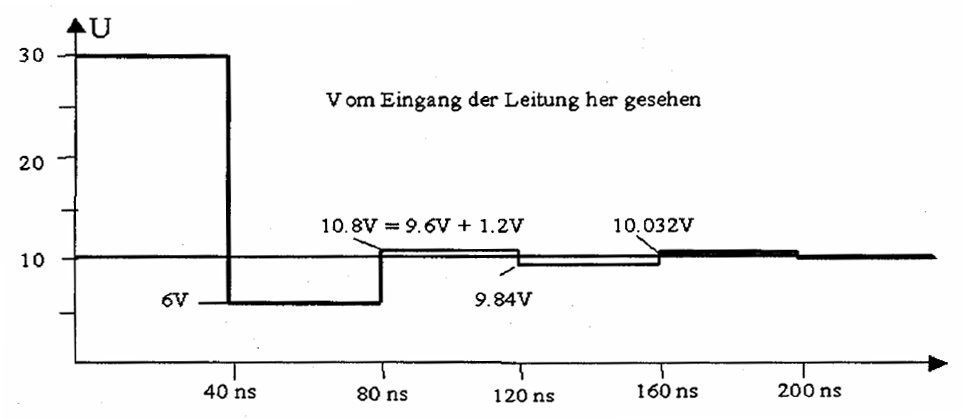
\includegraphics[height=4.1cm]{../El4/bilder/Leitungen_MFReflx_EnAP_SnAP_Eingangsspannung.png}      	
	    \end{minipage}
	\end{tabular}

    


\section{Smith Chart}
	\textbf{Nur für verlustlose Leitungen anwendbar!}
\subsection{Eigenschaften}
	\begin{tabular}{p{11cm}p{8cm}}
		\begin{minipage}{10cm}
        	\begin{itemize}{\setlength{\itemsep}{0cm}\setlength{\parsep}{0cm} \setlength{\topsep}{0cm}}
              \item \textbf{Normieren:} $\underline{Z}_{\text{einzutragen}} = \underline{Z}_N := \frac{Z}{R_0} = R_N + j X_N = \frac{\underline{r}+1}{\underline{r}-1}$
              \item $\underline{r}$ aus Smith-Chart; Da $ \underline{r} = \frac{\underline{Z}_N-1}{\underline{Z}_N+1} \rightarrow$ abhängig von $R_0$!
              \item \textbf{Impedanz $\Leftrightarrow$ Admittanz:} Am Kreismittelpunkt spiegeln \\
              $\underline{Y}_N = \frac{1}{\underline{Z}_N} \rightarrow \underline{r}_{Y_N} = -\underline{r}_{Z_N}$
              \item \textbf{Kurzschluss:} 	\textcolor{yellow}{Impedanz} \textcolor{orange}{Admittanz}
              \item \textbf{Leerlauf:}		\textcolor{orange}{Impedanz} \textcolor{yellow}{Admittanz}
        	  \item \textbf{Phase:}\\	In der Verlängerung der Reflexionsgerade am Kreisrand ablesen
        	  \item \textbf{VSWR:} Schnittpunkte von Kreis $\underline{r}$ mit reeller Achse bilden $R_1$ \& $R_2 \Rightarrow VSWR = \sqrt{\frac{R_2}{R_1}}$ 
        	  \item \textbf{gespiegelter Kreis:} Kreis mit konstantem Realanteil(=1) ($R_N/G_N =1$) gespiegelt an Mittelpunkt (''Einheitskreis'' in linker Ebene)
        	  \item \textbf{Leitungstransformation:} 
        	  Zeiger um modulo$0.5\left(\frac{l}{\lambda}\right)$ drehen. Richtung und Wert gemäss äusserster Skala $\frac{l}{\lambda}$
        	  \item \textbf{Addition von parallelen Leitungen}\\
        	  	Darauf achten, dass gleiches $R_0$! und Admittanzen addieren
        	  \item \textbf{Wellenwiderstandssprung}\\
        	  		Beim Widerstandssprung umnormieren!
        	   \item \textbf{Umnormieren:} $\underline{Z}_{N_{R_1}} = \underline{Z}_{N_{R_0}}\frac{R_0}{R_1}$
        	  \item \textbf{Entnormieren:}\\ $\underline{Z}_{\text{gewünscht}} = R_0
        	  \underline{Z}_{\text{abgelesen}} \qquad \underline{Y}_{\text{gewünscht}} = \frac{1}{R_0}
        	        \underline{Y}_{\text{abgelesen}}$
        	 
            \end{itemize}
            
        \end{minipage} &
		\begin{minipage}{8cm}
        	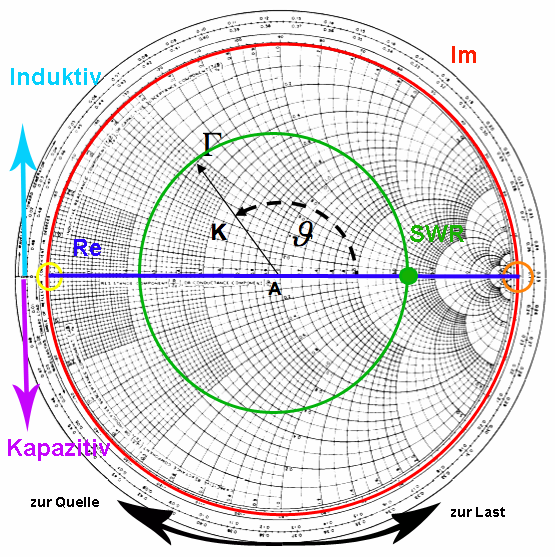
\includegraphics[height=7cm]{./bilder/SmithChart2.png}\\ \\
        	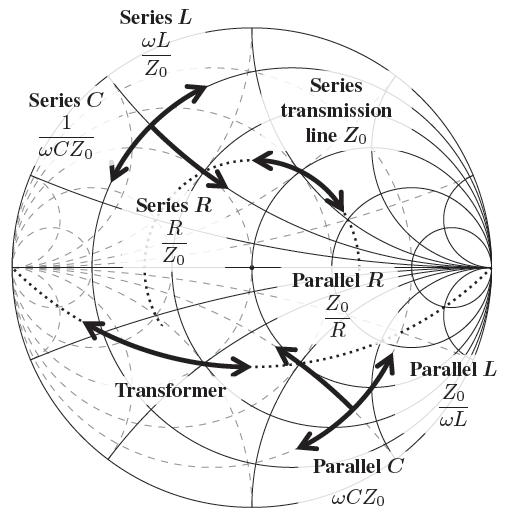
\includegraphics[height=7cm]{./bilder/smith_anpassung.png}
        \end{minipage}
	\end{tabular}
	
	
	\subsection{Anpassungen mit Smith-Chart}
	\begin{multicols}{2}
		\subsubsection{Anpassung durch Längs- und Querreaktanz}
			\parbox[c]{5cm}{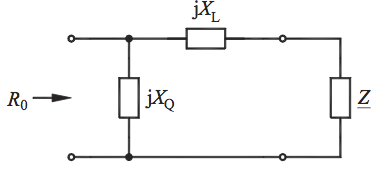
\includegraphics[width = 5cm]{./bilder/Anp_Laengs_Querreaktanz}} \parbox[c]{4cm}{Mit Längsreaktanz auf gespiegelten Kreis (Impedanzebene)}\\
			Auf Fehlabschlüsse mit $Re(\underline{Z}_N)<1$ beschränkt.
		\subsubsection{Anpassung durch Quer- und Längsreaktanz}
			\parbox[c]{5cm}{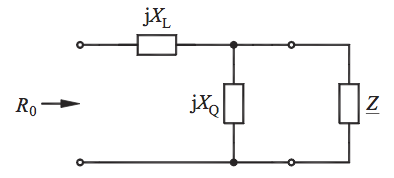
\includegraphics[width = 5cm]{./bilder/Anp_Quer_Laengsreaktanz}}
			\parbox[c]{4cm}{Mit Querreaktanz auf gespiegelten Kreis (Admittanzebene)}\\
			Auf Fehlabschlüsse mit $Re(\underline{Z}_N)>1$ beschränkt.
			\columnbreak
		\subsubsection{Anpassung durch Leitungsstück und Längsreaktanz}
			\parbox[c]{4.5cm}{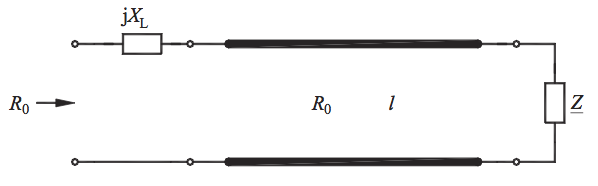
\includegraphics[width = 4.5cm]{./bilder/Anp_Leitung_Laengsreaktanz}
			Durch Leitungsstück auf $Re(\underline{Z}_N)=1$-Kreis transformieren (Impedanzebene)} \hspace{0.5cm}
			\parbox[c]{4.5cm}{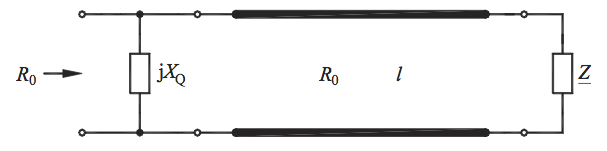
\includegraphics[width = 4.5cm]{./bilder/Anp_Leitung_Querreaktanz}
			Durch Leitungsstück auf $Re(\underline{Y}_N)=1$-Kreis transformieren (Admittanzebene)}
		\subsection{Anpassung durch $\lambda/4$-Transformation}
			\parbox[c]{5cm}{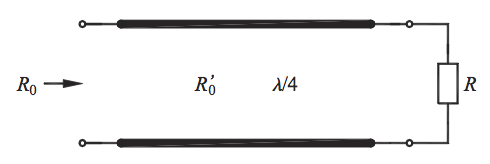
\includegraphics[width = 5cm]{./bilder/Anp_lambda_4_Transfor}}
			\parbox[c]{4cm}{$\frac{R}{R_0'}= \frac{R_0'}{R_0}$\\
			$\Rightarrow R_0' = \sqrt{R \cdot R_0}$}\\
			
	
	\end{multicols}
	
%\subsection{Beispiele bei $Z_0=100\Omega$}
%		\renewcommand{\arraystretch}{1.1}
%		\begin{tabular}{| c | c | c | c | c | c |}
%			\hline
%				\textbf{Fall}
%				& 1
%				& 2 
%				& 3
%				& 4
%				& 5 \\
%			\hline
%				\textbf{LE}
%				& Anpassung
%				& Leerlauf
%				& Kurzschluss
%				& $\lambda/8$ Stichleit. KS
%				& $\lambda/8$ Stichleit. LL \\
%			\hline
%				\textbf{SWR}
%				& 1
%				& $\infty$
%				& $\infty$
%				& $\infty$
%				& $\infty$ \\
%			\hline
%				\textbf{$\underline{r}$}
%				& $0$
%				& $1 \angle 0 ^\circ$
%				& $1 \angle 180 ^\circ$
%				& $1 \angle 90 ^\circ$
%				& $1 \angle 90 ^\circ$\\
%			\hline
%				\textbf{$\underline{Z}_N$}
%				& $1+j0$
%				& $\infty+j\infty$
%				& $0+j0$
%				& $0+j1$
%				& $0-j1$ \\
%			\hline
%				\textbf{$v_{xm}$}
%				& $-$
%				& $\lambda/4$
%				& $\lambda/2$
%				& $3\lambda/8$
%				& $\lambda/8$ \\
%			\hline
%				\textbf{Grafik}
%				& 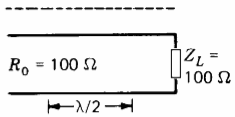
\includegraphics[height=0.9cm]{./bilder/Fall1.png}
%				& 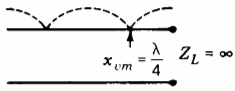
\includegraphics[height=0.9cm]{./bilder/Fall2.png}
%				& 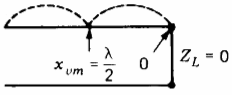
\includegraphics[height=0.9cm]{./bilder/Fall3.png}
%				& 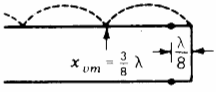
\includegraphics[height=0.9cm]{./bilder/Fall4.png}
%				& 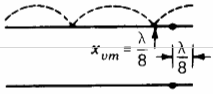
\includegraphics[height=0.9cm]{./bilder/Fall5.png} \\
%			\hline
%		\end{tabular}
%		\renewcommand{\arraystretch}{1}
		
\newpage

%
\section{Elektromagnetische Felder}
	\subsection{Elektromagnetische Wellenausbreitung}
		
		\begin{minipage}{4.3cm}
			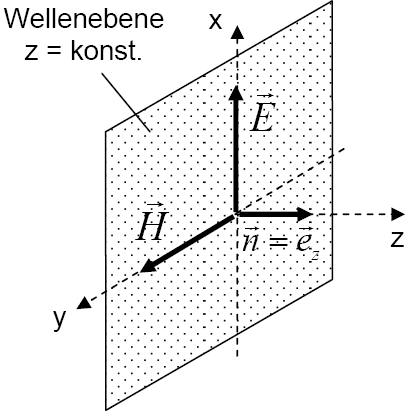
\includegraphics[width=4cm]{./bilder/EMW_EbeneWelle.png} 
        \end{minipage}
		\renewcommand{\arraystretch}{1.6}
		\begin{tabular}{| c | c | c | }
			\hline
				\multicolumn{3}{| c |}{\textbf{Definition Ebenen}}    \\
			\hline
				\multicolumn{3}{| l |}{\textbf{Wellenebene: } Durch $\vec{H}$ und $\vec{E}$ aufgespannt.} \\
				\multicolumn{3}{| l |}{\textbf{Trennebene: } Grenzfläche zwischen den beiden Medien.} \\ 
				\multicolumn{3}{| l |}{\textbf{Einfallsebene: } Durch Richtungsvektor der Wellenausbreitung
				und $\vec{n}_{Trennebene}$ aufgespannt.} \\
			\hline
    		\hline
				\textbf{Wellenwiderstand} & \textbf{Wellenwid.} - Vakuum & \textbf{Wellengeschwindigkeit,
				-konstante}\\
			\hline
				$Z=\dfrac{E}{H}=\sqrt{\frac{\mu}{\varepsilon}}$ 
				& $Z_0 = \sqrt{\frac{\mu_0}{\varepsilon_0}} = 120\pi \Omega$
				& $v=\frac{1}{\sqrt{\mu \varepsilon}} \quad v_0 = c\approx 3*10^8 \frac{m}{s}; \qquad \beta =
				\omega \sqrt{\mu \epsilon}$
				\\
			\hline
				\textbf{Orientierung} & \textbf{Poynting Vektor} & \textbf{Konstanten} \\
			\hline
				$Z \cdot \vec{H} = \vec{n} \times \vec{E}$
				& $\vec{S}=\vec{E}\times\vec{H}$
				& $\varepsilon_0=8,854\cdot 10^{-12}[\frac{As}{Vm}] \quad
				\mu_0=4\pi\cdot 10^{-7}[\frac{Vs}{Am}]$ \\
			\hline
			\hline
				\multicolumn{3}{| c |}{\textbf{Gebräuchliche Indizes}} \\
			\hline	
				\textbf{i}: incident = einfallend
				& \textbf{r}: reflected = reflektiert
				& \textbf{t}: transmitted = übermittelt 	\\
			\hline
   		\end{tabular}
		\renewcommand{\arraystretch}{1}


		
	\subsubsection{Leitender Halbraum}	
		Die Welle wird an der Trennebene vollständig reflektiert. \\
				
		\begin{minipage}{4cm}
			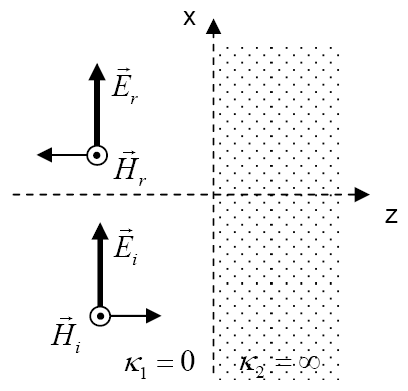
\includegraphics[width=3.8cm]{./bilder/EMW_LHR_SenkrechtEinfallendeWelle.png} 
        \end{minipage}
		\renewcommand{\arraystretch}{1.6}
		\begin{tabular}{| l  | l |}
			\hline
				\multicolumn{2}{|l|}{\textbf{Senkrecht einfallende Ebene Welle}} \\		
				\hline
				$E_r + E_i = 0 \Rightarrow E_r = - E_i$ & \\
				$\vec{E}_i (z) = \vec{e}_x E_i e^{-j \beta_1 z} \qquad  \qquad 
				\vec{E}_r (z) = \vec{e}_x E_r e^{+j \beta_1 z}$
				
				& $\vec{H}_i (z) = \vec{e}_y \frac{E_i}{Z_1} e^{-j \beta_1 z} \qquad  \qquad 
				\vec{H}_r (z) = \vec{e}_y \frac{E_i}{Z_1} e^{+j \beta_1 z}$
				\\
				
				$\vec{E}_1 (z) = \vec{e}_x E_i (e^{-j \beta_1 z} - e^{+ j \beta_1 z}) = 
				-\vec{e}_x j 2 E_i \sin{(\beta_1 z)}	$
				& 
				$\vec{H}_1 (z) = \vec{e}_y \frac{E_i}{Z_1} (e^{-j \beta_1 z} + e^{+ j \beta_1 z}) = 
				\vec{e}_y j 2 \frac{E_i}{Z_1} \cos{(\beta_1 z)}	$ \\
				
				$E_1 (z,t) = \text{Re}\left\{ \vec{E}_1(z) e^{j \omega t}\right\} =
				\vec{e}_x 2 E_i \sin{(\beta_1 z)} \sin{(\omega t)}	$
				& 
				$H_1 (z,t) = \text{Re}\left\{ \vec{H}_1(z) e^{j \omega t}\right\} =
				\vec{e}_y 2 \frac{E_i}{Z_1} \cos{(\beta_1 z)} \cos{(\omega t)}	$\\		
				
			\hline
   		\end{tabular}
		\renewcommand{\arraystretch}{1}	
		
		\begin{minipage}{4.3cm}
			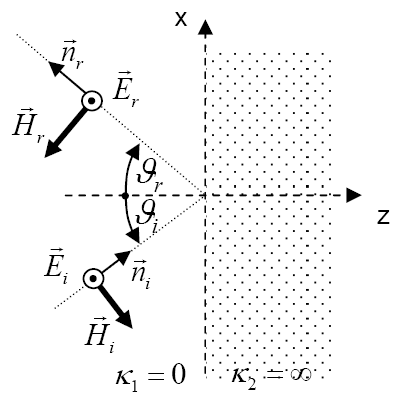
\includegraphics[width=4cm]{./bilder/EMW_LHR_SchraegSenkrechtPolarisiert.png} 
        \end{minipage}
		\renewcommand{\arraystretch}{1.6}
		\begin{tabular}{| c || c | }
			\hline
				\multicolumn{2}{|c|}{\textbf{Schräg einfallende Welle}} \\
			\hline
				\textbf{Senkrechte Polarisation}
				& 
				\textbf{Parallele Polarisation} \\	
			\hline		
				$\vec{E} \perp $ Einfallsebene
				& 
				$\vec{E} \parallel $ Einfallsebene \\
			\hline	
 				$\vec{n}_i = \vec{e}_x \sin(\vartheta_i)+\vec{e}_z \cos(\vartheta_i)$&\\
 				$\vec{n}_r=\vec{e}_x \sin(\vartheta_i)- \vec{e}_z \cos(\vartheta_i)$ &\\
  				$\vec{r}=\vec{e}_x x+\vec{e}_z z;$ 
 				$E_r=-E_i; \vartheta_r =\vartheta_i$&\\
 				$\vec{E}_{i(x,z)} =\vec{e}_y E_i e^{-j \beta_1 \vec{n}_i \vec{r}}$&\\ 
 				$\vec{E}_r(x,z) =\vec{e}_y E_i e^{-j \beta_1 \vec{n}_r
 				\vec{r}}=- \vec{e}_y E_i e^{-j \beta_1
 				(x\sin(\vartheta_i)-z\cos(\vartheta_i))}$&\\
 				$\vec{H}_{r(x,z)}=\frac{1}{z_1}(\vec{n}_r\times \vec{E}_{r(x,z)})$&\\
 				\hline
 				\multicolumn{2}{|l|}{
				$\vec{n_i}=
				\frac{\beta_x}{\beta}\vec{e}_x + \frac{\beta_y}{\beta} \vec{e}_y + 
				\frac{\beta_z}{\beta} \vec{e}_z
				\qquad \qquad \beta=\sqrt{\beta_x^2+\beta_y^2+\beta_z^2}$}\\
			\hline
   		\end{tabular}
		\renewcommand{\arraystretch}{1}	
		\begin{minipage}{4.3cm}
			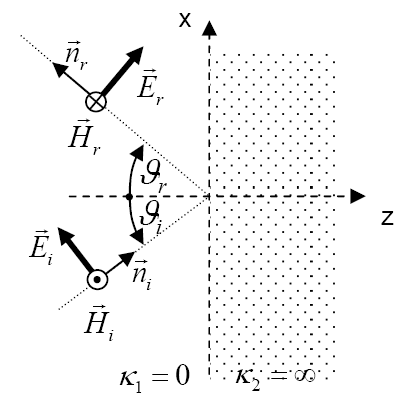
\includegraphics[width=4cm]{./bilder/EMW_LHR_SchraegParallelPolarisiert.png} 
        \end{minipage}	

	\subsubsection{Dielektrischer Halbraum}
		Je nach Einfallswinkel $\vartheta_i$ wird die Welle nicht nur reflektiert, sondern dringt in das
		zweite Medium ein. \\
		
		\renewcommand{\arraystretch}{1.6}
		\begin{tabular}{| l  | l | l |}
			\hline
				\textbf{Transmissionskoeffizient} & \textbf{Reflexionskoeffizient} &
				\textbf{Stehwellenverhältnis}
				\\
			\hline
				$t = \dfrac{E_t}{E_i} = \dfrac{2 Z_2}{Z_2 + Z_1} \qquad 1 + r = t$ 
				& $r = \dfrac{E_r}{E_i} = \dfrac{Z_2 - Z_1}{Z_2 + Z_1} \qquad  |r| = \dfrac{SWR - 1}{SWR + 1}$
				& $SWR = \dfrac{|E|_{max}}{|E|_{min}} = \dfrac{1 + |r|}{1 - |r|}$ \\
			\hline
   		\end{tabular}
		\renewcommand{\arraystretch}{1}	
		
		\begin{minipage}{4cm}
			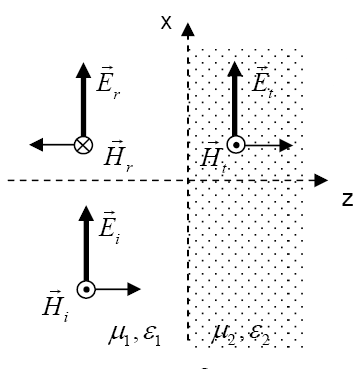
\includegraphics[width=4cm]{./bilder/EMW_DHR_SenkrechtEinfallendeWelle.png} 
        \end{minipage}
		\renewcommand{\arraystretch}{1.6}
		\begin{tabular}{| l  | l |}
			\hline
				\multicolumn{2}{|c|}{\textbf{Senkrecht einfallende Ebene Welle}} \\
			\hline
				$E_i + E_r = E_t$ &
				$H_i + H_r = H_t$ \\
			\hline
   		\end{tabular}
		\renewcommand{\arraystretch}{1}	
		
				
		
		
		\begin{minipage}{4.3cm}
			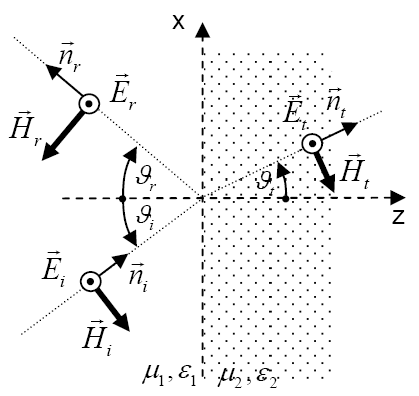
\includegraphics[width=4cm]{./bilder/EMW_DHR_SchraegSenkrechtPolarisiert.png} 
        \end{minipage}
		\renewcommand{\arraystretch}{1.6}
		\begin{tabular}{| c || c | }
			\hline
				\multicolumn{2}{|c|}{\textbf{Schräg einfallende Welle}} \\
			\hline
				\multicolumn{2}{|c|}{$\dfrac{\sin{\vartheta_t}}{\sin{\vartheta_i}} = \sqrt{\dfrac{\mu_1
				\epsilon_1}{\mu_2 \epsilon_2}} \qquad \vartheta_r = \vartheta_i$} \\
			\hline
				\textbf{Senkrechte Polarisation}
				& 
				\textbf{Parallele Polarisation} \\	
			\hline		
				$ \sin^2 \vartheta_{Brewster_1} = \dfrac{1 - \frac{\mu_1 \epsilon_2}{\mu_2 \epsilon_1}}{1 -
				\left(\frac{\mu_1}{\mu_2}\right)^2}$ 
				& $ \sin^2 \vartheta_{Brewster_2} = \dfrac{1 - \frac{\mu_2 \epsilon_1}{\mu_1 \epsilon_2}}{1 -
				\left(\frac{\epsilon_1}{\epsilon_2}\right)^2}$ \\
				$r_{SP} = \dfrac{E_r}{E_i} = \dfrac{Z_2 \cos{\vartheta_i} - Z_1 \cos{\vartheta_t}}{Z_2
				\cos{\vartheta_i} + Z_1 \cos{\vartheta_t}}$
				& $r_{PP} = \dfrac{E_r}{E_i} = \dfrac{Z_2 \cos{\vartheta_t} - Z_1 \cos{\vartheta_i}}{Z_2
				\cos{\vartheta_t} + Z_1 \cos{\vartheta_i}}$ \\
				$t_{SP} =  \dfrac{E_t}{E_i} = \dfrac{2 Z_2 \cos{\vartheta_i}}{Z_2 \cos{\vartheta_i} + Z_1
				\cos{\vartheta_t}}$
				& $t_{PP} = \dfrac{E_t}{E_i} =  \dfrac{2 Z_2 \cos{\vartheta_t}}{Z_2 \cos{\vartheta_t} + Z_1
				\cos{\vartheta_i}}$ \\
			\hline
   		\end{tabular}
		\renewcommand{\arraystretch}{1}	
		\begin{minipage}{4.3cm}
			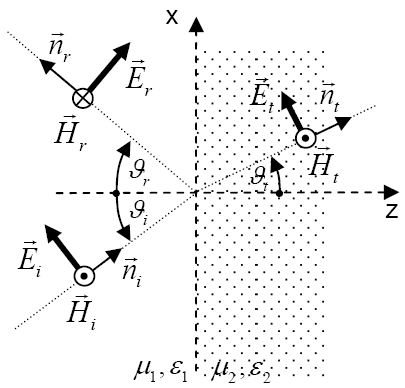
\includegraphics[width=4cm]{./bilder/EMW_DHR_SchraegParallelPolarisiert.png} 
        \end{minipage}	
		
	\subsection{Hertz'scher Dipol}		
		\begin{minipage}{4.8cm}
			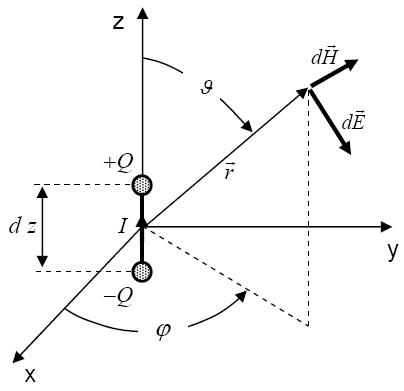
\includegraphics[height=4.7cm]{./bilder/LinAnt_HerzscherDipol.png}
        \end{minipage}
		\renewcommand{\arraystretch}{1.6}
		\begin{tabular}{| c | c | c | c |}
    		\hline
    	\multicolumn{2}{| c |}{\textbf{Magnetische Feld}} & \multicolumn{2}{| c
    	|}{\textbf{Wellenwiderstand}} \\
    		\hline
    	\multicolumn{2}{| c |}{$\vec{H} = \vec{e}_{\varphi} \dfrac{j \beta \sin \vartheta}{4 \pi r}
    	e^{-j \beta r} \int\limits_{-l}^{+l}I(z) e^{j \beta z \cos \vartheta} dz$}
    	& \multicolumn{2}{| c |}{$Z_0 = \dfrac{dE}{dH} \sqrt{\dfrac{\mu_0}{\epsilon_0}}$}
    	\\
			\hline
    	\multicolumn{4}{| c |}{\textbf{Fernfeld} - ($\beta z = 2 \pi z / \lambda \ll 1$)} \\        
    		\hline
    	\multicolumn{2}{| c |}{$\vec{H} = \vec{e}_{\varphi} \dfrac{I_0 l \sin \vartheta}{4 \pi r} j
    	\beta e^{-j \beta r} $} 
    	& \multicolumn{2}{| c |}{$\vec{E} = \vec{e}_{\vartheta} Z_0 \dfrac{I_0 l \sin \vartheta}{4
    	\pi r} j \beta e^{-j \beta r} $}\\
			\hline
    		\hline   
    	\multicolumn{2}{| c |}{\textbf{Strahlungsleistung}} & \textbf{Strahlungswid.} &
    	\textbf{Strahlungschar.} \small{($\Phi_0 = \Phi(\frac\pi2)$)}  \\
    		\hline
    	\multicolumn{2}{| c |}{$\bar{P}_s = \dfrac{2 \pi}{3} Z_0 \left( \dfrac{l}{\lambda}\right)^2
    	I_0^2 = 
    	\dfrac{1}{2}
    	\text{Re} \left\{ \oiint\limits_{F \infty} (\vec{E}
    	\times
    	\vec{H}^* ) d \vec{F} \right\}  $}
    	& $R_s=\frac{2\pi}{3}Z_0 \left(\frac{l}{\lambda}\right)^2$
    	& $\Phi(\vartheta) = \dfrac{Z_0}{4} \left( \dfrac{l}{\lambda} \right)^2 I_0^2
    	\sin^2\vartheta$
    	\\
		\hline
   		\end{tabular}
		\renewcommand{\arraystretch}{1}
	
		
	\subsection{Lineare Antennen}
		\begin{minipage}{2.2cm}
			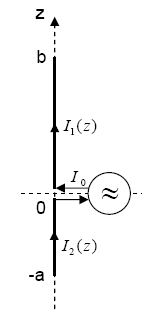
\includegraphics[height=4.5cm]{./bilder/LinAnt_Stromverteilung.png}
        \end{minipage}
		\begin{minipage}{12.7cm}
		\renewcommand{\arraystretch}{1.6}
		\begin{tabular}{| c | c |}
    		\hline
    	\multicolumn{2}{| c |}{\textbf{Strahlung linearer Antennen} - siehe Bild rechts} \\        
    		\hline
    $\vec{H}(\vec{r}_P) = - \frac{j}{2 \lambda r_p} e^{-j 2 \pi \frac{r_p}{\lambda}}     
    \int\limits_A^B I(\vec{r}_Q) e^{j 2 \pi \frac{\vec{n} \vec{r}_Q}{\lambda}} (\vec{n} \times
    d \vec{r}_Q) $
	&
    $ \vec{E}(\vec{r}_p) = - Z_0 \left[ \vec{n} \times \vec{H} (\vec{r}_p) \right] $
    \\
			\hline
    		\hline   
    	\multicolumn{2}{| c |}{\textbf{Strahlungscharakteristik}}
    	\\
    		\hline
    \multicolumn{2}{| c |}{$ \Phi(\vec{n}) = \dfrac12 Z_0 r_P^2 \vec{H} (\vec{r}_p) \cdot \vec{H}^*
    (\vec{r}_p) = \vec{n} r^2_p \bar{S}(\vec{r}_p) = \dfrac{1}{2} \vec{n} r_p^2 \text{Re} \left\{
    -Z_0 ( \vec{n} \times \vec{H} ) \times \vec{H}^* \right\} $} \\
			\hline
    		\hline
    	\multicolumn{2}{| c |}{\textbf{Stromverteilung auf linearen Antennen} - siehe Bild links} \\
    		\hline
    	$ I_1 (z) = \dfrac{\sin{[\beta (b - z)]}}{\sin{[\beta b]}} I_0 ; \quad 0 \leq z \leq
    	b$
    	& 
    	$ I_2 (z) = \dfrac{\sin{[\beta (a + z)]}}{\sin{[\beta a]}} I_0 ; \quad -a \leq z \leq
    	0$ \\
    	
    		\hline
    		\hline
    	\textbf{Strahlungsleistung} & \textbf{Strahlungswiderstand} \\
    		\hline
    	$ \bar{P}_S = \int\limits_0^{2\pi}\int\limits_0^{\pi} \Phi(\vartheta) \sin \vartheta \cdot
    	d \vartheta \cdot d \varphi	$ 
    	& 
    	$ R_S = \dfrac{2}{I_0^2 } \int\limits_0^{2\pi}\int\limits_0^{\pi} \Phi(\vartheta) \sin \vartheta \cdot
    	d \vartheta \cdot d \varphi	$ \\
    		\hline
   		\end{tabular}
		\renewcommand{\arraystretch}{1}
        \end{minipage}		
		\begin{minipage}{4.5cm}
			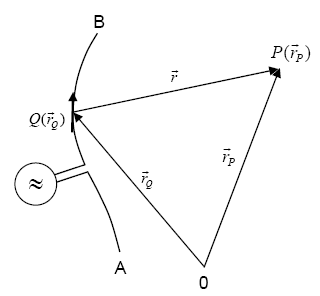
\includegraphics[height=4cm]{./bilder/LinAnt_Strahlung.png}
        \end{minipage}
		
	\subsubsection{Richtcharakteristika}
	\begin{center}
		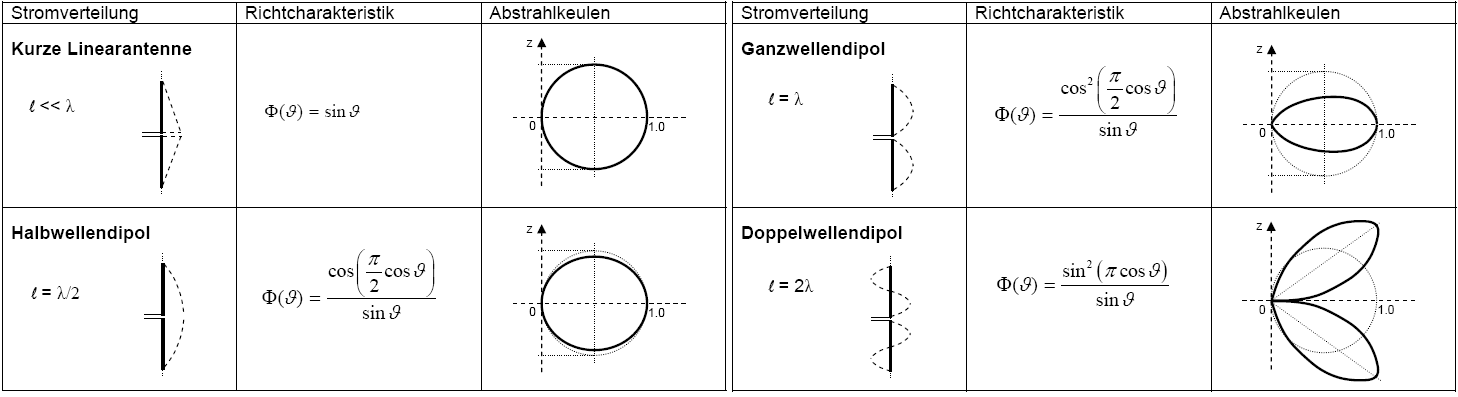
\includegraphics[width=19cm]{./bilder/LinAnt_Richtcharakteristika.png}    
  \end{center}

  \section{Integral-Gesetze der Elektrotechnik}
	\renewcommand{\arraystretch}{2}
	\begin{tabular}{|p{2.5cm}||p{2.7cm}|p{4cm}|p{2.7cm}|p{5cm}|}
	\hline
	& \textbf{Elektr. Feld} & \textbf{Magn. Feld} & \textbf{Strömungsfeld} & \textbf{Bemerkung}\\
	\hline \hline
	Feldgrösse & $\vec{E}$, $\vec{D}$ & $\vec{H}$, $\vec{B}$
	& $\vec{E}$, $\vec{J}$ &\\
	\hline
	Konstante
		& \parbox{2.7cm}{$\varepsilon_0 = 8.854 \cdot 10^{-12}$\\
		{\tiny Dielektrizitätskonstante} \vspace{.1cm}} 
		& \parbox{4cm}{$\mu_0 = 4 \pi \, 10^{-7}$\\ {\tiny Permeabilitätskonstante} \vspace{.1cm}} 
		& \parbox{2.7cm}{$\sigma=\frac{1}{\rho}$ \\ {\tiny Spezifische
		Leitfähigkeit}\vspace{.1cm}} &\\ 
	\hline
	Stoffgleichung & $\vec{D}=\varepsilon_0\varepsilon_r\vec{E}$ & $\vec{B}=\mu_0\mu_r\vec{H}$
	& $\vec{J}=\sigma\vec{E}$ &
	\\
	\hline
	Kraft & $\vec{F_C}=q\vec{E}$ & $\vec{F_L}=q(\vec{v}\times\vec{B})$ &&\\
	\hline
	\parbox{2.5cm}{Fluss\\{\tiny (durch Fläche A)}} & $\Psi_{el}=\int\vec{D}\vec{dA}$ &
	$\Phi_m=\int\vec{B}\vec{dA}$ \textsuperscript{1)}&
	$I=\int\vec{J}\vec{dA}$ & \textsuperscript{1)} bei Spulen:
	$\Psi_m=\sum_i\Phi_i\approx N \Phi$\\
	\hline
	\parbox{2.5cm}{Spannung \\{\tiny (Weg A$\to$B)}} & $U_{AB}=\int\limits_{A}^B
	\vec{E}\vec{ds}$ & $V_{m_{AB}}=\int\limits_{A}^B\vec{H}\vec{ds}$ 
	& $U_{AB}=\int\limits_{A}^B\vec{E}\vec{ds}$ & \\
	\hline
	Schaltelemente & $Q=CU$ & $\Psi_m=LI$, $\Psi_{m21}=M_{21}I_1$
	& $I=GU$, $U=RI$ & $R_m=\frac{1}{\Lambda}$, $R=\frac{1}{G}$\\
	\hline
	\parbox{2.5cm}{Hüllengesetz \\ {\tiny (Quellengleichungen)}}
		& \parbox{2.7cm}{
			\vspace{.1cm}$\oint\vec{D}\vec{dA}=\sum Q_i$ \vspace{.1cm}
			Maxwell IV
			\vspace{.1cm}}
		& \parbox{4cm}{
			\vspace{.1cm}$\oint\vec{B}\vec{dA}=0$
			\textsuperscript{2)} \\
			Maxwell III
			\vspace{.1cm}} 
		& \parbox{2.7cm}{
			$\oint\vec{J}\vec{dA}=0$\\
			Kirchhoff 1}
		& \parbox{5cm}{\textsuperscript{2)} ohne Verschiebungsstrom (käme ggf. noch
		dazu)} \\
	\hline
	Umlaufspannung 
		& \parbox{2.7cm}{
			\vspace{.1cm}
			$\oint\vec{E}\vec{ds}=0-\dot{\Phi}_m$ \\ 
			{\tiny Induktionsgesetz}\\Maxwell II
			\vspace{.1cm}}
		& \parbox{4cm}{
			\vspace{.1cm}
			$\oint\vec{H}\vec{ds}=\theta+\dot{\Psi}_{el}$ \\ 
			{\tiny Vollständiges Durchflutungsgesetz} \\Maxwell I
			\vspace{.1cm}}
		& \parbox{2.7cm}{
			\vspace{.1cm}
			$\oint\vec{E}\vec{ds}=0-\dot{\Phi}$ \\ Kirchhoff 2
			\vspace{.1cm}}
		& \\
	\hline
	\end{tabular}
	\renewcommand{\arraystretch}{1} \\

\textbf{Einheiten}\\
\renewcommand{\arraystretch}{1.2}
	\begin{tabular}{|l|l|l|l|l|l|}
	\hline
	$[\varepsilon] = \frac{As}{Vm}$
		& $[D] = \frac{As}{m^2} = \frac{C}{m^2}$
		& $[E] = \frac{V}{m}$
		& $[U] = V$
		& $[\Psi_{el}] = As = C$
		& $[C] = F$ \\
	\hline
	$[\mu] = \frac{H}{m}=\frac{V s}{A m}$
		& $[B] = \frac{Vs}{m^2} = T$
		& $[H] = \frac{A}{m}$
		& $[V_m] = [\Theta] = A$
		& $[\Psi_m] = [\Phi_m] = Wb = Vs$
		& $[L] = \frac{Vs}{A} = H$ \\
	\hline
	$[\sigma] = \frac{S}{m}$
		& $[E] = \frac{V}{m}$
		& $[J] = \frac{A}{m^2} = 10^{-6} \frac{A}{mm^2}$
		& $[U] = V$
		& $[I] = A$
		& $[R] = \Omega$ \\
	\hline
	\end{tabular}
	\renewcommand{\arraystretch}{1}
%\newpage


\section{Allgemein}
	\subsection{Schaltelemente bei zeitabhängigen Vorgängen}
	\begin{tabular}{p{1.5cm} p{4.3cm} p{1.5cm} p{4.3cm} p{1.5cm} p{4.3cm}}
   		\multicolumn{2}{l}{\textbf{Ohmscher Widerstand R}}
   			& \multicolumn{2}{l}{\textbf{Kapazitität C}}
   			& \multicolumn{2}{l}{\textbf{Induktivität L}} \\
   		\multicolumn{2}{l}{$u$ und $i$ können sprunghaft ändern}
   			& \multicolumn{2}{l}{$u$ kann nicht sprunghaft ändern}
   			& \multicolumn{2}{l}{$i$ kann nicht sprunghaft ändern} \\
   		\parbox{1.5cm}{
			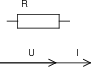
\includegraphics[width=1.5cm]{./bilder/zeigerdiag-r.png}}
			& \parbox{4.3cm}{$u(t) = R i(t)$ \\
				$i(t) = \frac{u(t)}{R}$ \\
				$\underline{Z} = R$}
   			& \parbox{1.5cm}{
				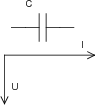
\includegraphics[width=1.5cm]{./bilder/zeigerdiag-c.png}}
			& \parbox{4.3cm}{
				$u(t) = \frac1C \int\limits_0^t i(\tau) d\tau + u(0)$ \\
				$i(t) = C \frac{d u(t)}{dt}$ \\
				$\underline{Z} = \frac{1}{j \omega C} = - \frac{j}{\omega C}$ \\
				$W_C=\frac12 C U_C^2$}
   			& \parbox{1.5cm}{
				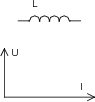
\includegraphics[width=1.5cm]{./bilder/zeigerdiag-l.png}}
			& \parbox{4.3cm}{
				$u(t) = L \frac{di(t)}{dt}$ \\
				$i(t) = \frac1L \int\limits_0^t u(\tau) d\tau + i(0)$ \\
				$\underline{Z} = j \omega L$ \\
				$W_L=\frac12 L I_L^2$}
   	\end{tabular}

	\subsection{Vorgehen bei Schaltvorgängen}
		\fbox{$u(t) =U_E + (U_A - U_E) e^{\frac{-t}{\tau}} \qquad \tau = C R \text{ bzw. }
		\tau =
		 \frac{L}{R} = \frac{\varepsilon}{\sigma} \qquad U_A = \lim\limits_{t
		 \rightarrow 0^+} u(t) \qquad U_E =
		 \lim\limits_{t \rightarrow \infty} u(t)$} $\qquad$ Für Ströme äquivalent
		 
		 \subsection{Taschenrechner TI-89/Voyage 200 englisch}
		 	\begin{tabular}{p{6cm} p{12cm}}
				 \texttt{comDenom(Z/N, x)} & Gemeinsamen Nenner finden \\
				 \texttt{cZeros($\ldots p^m \ldots$ | p = i * $\omega$, $\omega$)} &
				 Komplexe Nullstellen finden (für Pole jeweils Nenner der UTF einsetzen) \\
				 \texttt{expand($p^n/q^m$)} & Partialbruchzerlegung \\
				 \texttt{propFrac($p^n/q^m$)} & Polynomdivision \\
				 \texttt{pds$\backslash$partial($\{a_n, \ldots, a_0\},\{b_m, \ldots, b_0\}$)} & 100\%-ige
				 Partialbruchzerlegung, \textcolor{red}{Root-Folder}: Mode
				 $\rightarrow$ Current Folder $\rightarrow$ pds \\ 
				 \texttt{pds$\backslash$roots($\{a_n, \ldots, a_0\}$)} & Nullstellen
				 bestimmen \\ \texttt{acst$\backslash$laplace($f(t)$)} & Laplacetransformation \\
				 \texttt{acst$\backslash$invlap($F(s)$)} & inverse Laplacetransformation   
			\end{tabular}
		 
		 
	\subsection{Vektor -/ Kreuzprodukt, Rechte-Hand-Regel}
	$\vec{c} = \vec{a} \times \vec{b}$: \qquad $\vec{a} \Leftrightarrow$ Daumen;
	$\vec{b} \Leftrightarrow$ Zeigefinger; $\vec{c} \Leftrightarrow$ Mittelfinger
	 
	 \subsection{Partialbruchzerlegung\formelbuch{15}}
		Falls möglich, erst Polynomdivision.
		\[f(x)=\frac{x^2+20x+149}{x^3+4x^2-11x-30} \Rightarrow \; \begin{array}{l}\text{Nenner faktorisieren mit}\\
		\text{Hornerschema\formelbuch{914}, Binom, etc.}\end{array} \Rightarrow x^{3}+4x^{2}-11x-30=(x+2)(x^{2}+2x-15)=(8x+2)(x+5)(x-3)\]
		Ansatz:
		\[f(x)=\frac{x^2+20x+149}{x^3+4x^2-11x-30}=\frac{A}{x-3} + \frac{B}{x+2} + \frac{C}{x+5}=
		\frac{A(x+2)(x+5)+B(x-3)(x+5)+C(x-3)(x+2)}{(x-3)(x+2)(x+5)}\]
		Gleichungssystem aufstellen mit beliebigen $x_i$-Werten (am Besten Polstellen oder 0,1,-1 wählen):
		\[\begin{array}{l}x_1=3:\;-9+60+149=A\cdot5\cdot8\;\;\;\Rightarrow A=5\\
		x_2=-2:\;-4-40+149=B(-5)\cdot3\; \Rightarrow B=-7\\
		x_3=-5:\;-25-100+149=C(-8)(-3) \Rightarrow C=1 \end{array} \Rightarrow f(x)=\frac{5}{x-3}+\frac{7}{x+2}\frac{1}{x+5}\]
		weitere Ansätze für andere Typen von Termen:
		\[f(x)=\frac{5x^2-37x+54}{x^3-6x^2+9x}=\frac{A}{x}+\frac{B_1}{x-3}+\frac{B_2}{(x-3)^2}=\frac{A(x-3)^2+B_1x(x-3)+B_2x}{x(x-3)^2}\]
		\[f(x)=\frac{1,5x}{x^3-6x^2+12x-8}=\frac{A_1}{x-2}+\frac{A_2}{(x-2)^2}+\frac{A_3}{(x-2)^3}=\frac{A_1(x-2)^2+A_2(x-2)+A_3}{(x-2)^3}\]
		\[f(x)=\frac{x^2-1}{x^3+2x^2-2x-12}=\frac{A}{x-2}+\frac{Bx+C}{x^2+4x+6}=\frac{A(x^2+4x+6)+(Bx+C)(x-2)}{(x-2)(x^2+4x+6)}\]
	\subsection {Komplexe Trigonometrie}
\begin{tabular}{lllllll}
$\sin{\underline{\alpha}} = \frac{e^{j\underline{\alpha}} - e^{-j\underline{\alpha}}}{2j}$ &

$\cos{\underline{\alpha}} = \frac{e^{j\underline{\alpha}} + e^{-j\underline{\alpha}}}{2}$ &

$\tan{\alpha} = \frac{\sin \alpha}{\cos \alpha}$ & 

$ \qquad \qquad $ &

$\sinh{\underline{\alpha}} = \frac{e^{\underline{\alpha}} - e^{-\underline{\alpha}}}{2} $ &

$\cosh{\underline{\alpha}} = \frac{e^{\underline{\alpha}} + e^{-\underline{\alpha}}}{2} $ &

		$\tanh(jb)=j \tan(b)$ 
\end{tabular}
							
	 

\newpage
\end{document}
